\documentclass[final]{statsoc}


\usepackage[letterpaper]{geometry}
\usepackage{amsmath}
\usepackage{amssymb}
\usepackage{amsbsy}
\usepackage{epsfig}
\usepackage{color}
\usepackage{url}
\usepackage{dsfont}
\usepackage{bm}
\usepackage{multirow}

\title[Risk Mapping - Multiple Point Patterns]{Urban Heat Risk Mapping Using Multiple Point Patterns in Houston, Texas}
\author{Jacob W. Mortensen}
\address{Department of Statistics, Brigham Young University,
Provo, UT 84602,
United States.}
\email{jacob.w.mortensen@byu.edu}
\author[Heaton]{Dr. Matthew J. Heaton}
\address{Department of Statistics, Brigham Young University,
Provo, UT 84602,
United States.}
\author[Mortensen, Heaton \& Wilhelmi]{Olga V. Wilhelmi}
\address{Research Applications Laboratory, National Center for Atmospheric Research, 
Box 80307-3000, Boulder, CO,
United States.}



\begin{document}

\begin{abstract}
Extreme heat, or persistently high temperatures in the form of heat waves,
adversely impact human health. To study such effects, risk maps are a common
epidemiological tool used to identify regions and populations that are
more susceptible to these negative outcomes; however, the negative health 
effects of high temperatures are manifested differently among
different segments of the population. In this paper, we propose a novel,
hierarchical marked point process model that merges multiple health outcomes
into an overall heat risk map. Specifically, we consider health outcomes of  heat stress-related 911 calls and mortalities across the city of Houston, Texas. We show that combining multiple health outcomes leads to a broader
understanding of the spatial distribution of heat risk than a single 
health outcome.
\end{abstract}
\keywords{Poisson point processes, risk mapping}

\section{Introduction}
\subsection{Research Motivation}
Epidemiological evidence suggests that extreme or persistently high
temperatures negatively impact public health. For example, \cite{Basu2002},
\cite{Gosling2009}, \cite{Anderson2011} and \cite{Gasparrini2011}
have found that elevated temperatures increase mortality. Similarly,
empirical evidence suggests that increases in temperature are also 
related to increases in morbidity counts \citep{Li2012}, hospitalizations
\citep{Rusticucci2002,Schaffer2012} and ambulance
dispatches \citep{Ng2014}. As recently as 2015, heat waves in India 
and Pakistan contributed to the deaths of hundreds of people \citep{Mohsin2015}.
Studies by \cite{Luber2008}, \cite{Meehl2004}, \cite{Nicholls2009} and
\cite{Peng2011} suggest that, due to climate change, such negative
health outcomes are projected to increase in the future.

Risk (i.e. disease) mapping \citep{Lawson2013} is a common technique
used by epidemiologists to understand the spatial distribution
of those adversely affected by heat. However, \cite{Wilhelmi2010},
\cite{Wolf2010}, \cite{Uejio2011} and \cite{Heaton2014}
argue that the impact of heat on health is a multifaceted phenomenon that affects different 
segments of a population in different ways. For example, heat may lead to mortality
in some but dehydration in others. Thus, considering different health
outcomes can lead to different risk maps, each of which captures only a small
piece of the larger, cumulative impact of heat.

\begin{figure}
  \centering
  \begin{minipage}[t]{1.0\textwidth}
    \centering
    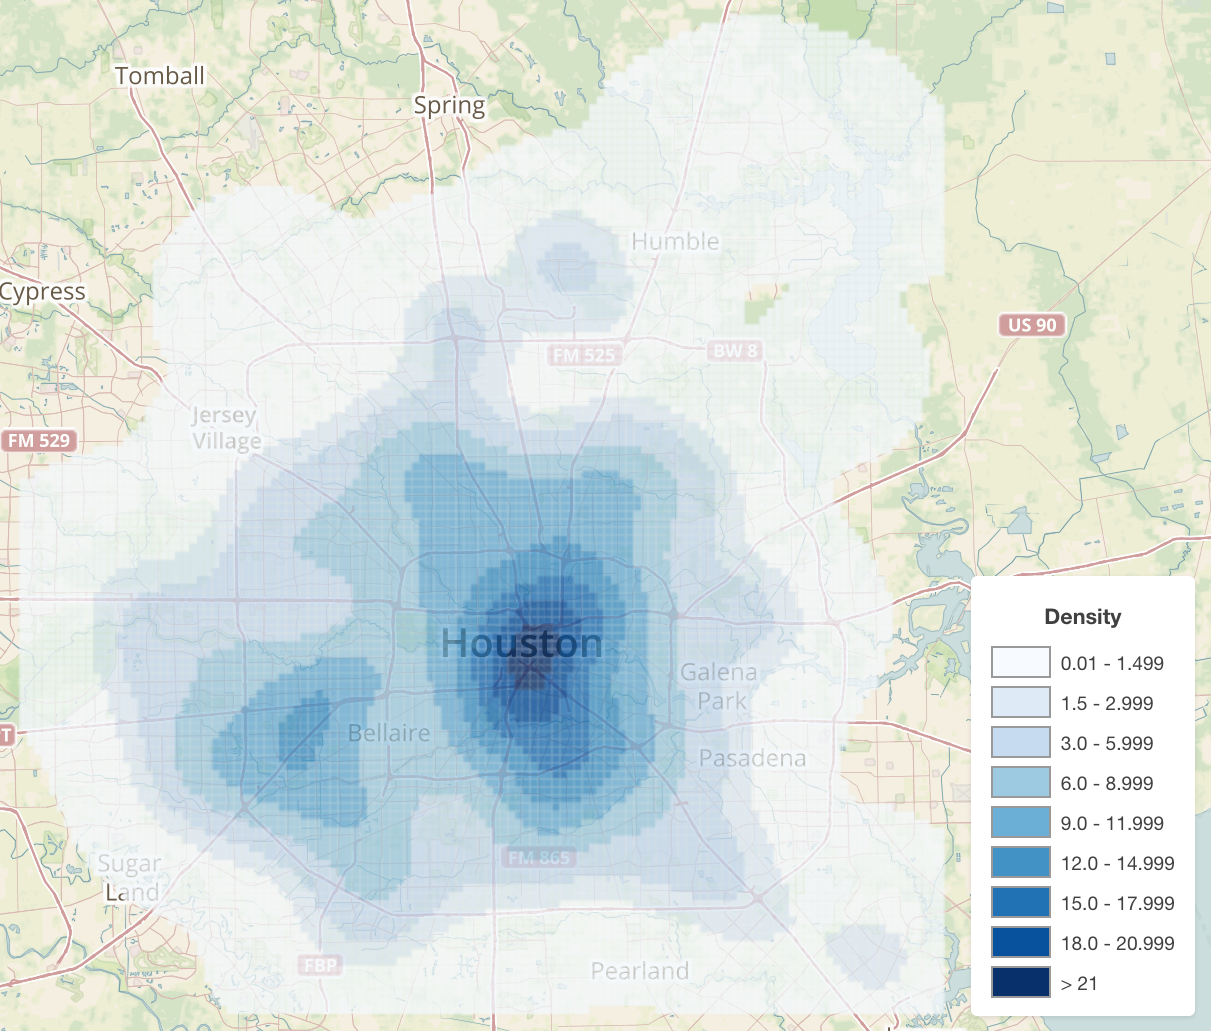
\includegraphics[width=0.7\textwidth]{./imgs/911_kde.png}
    \\
    a) 911 Data
    \\
  \end{minipage}
  \vfill
  \begin{minipage}[t]{1.0\textwidth}
    \centering
    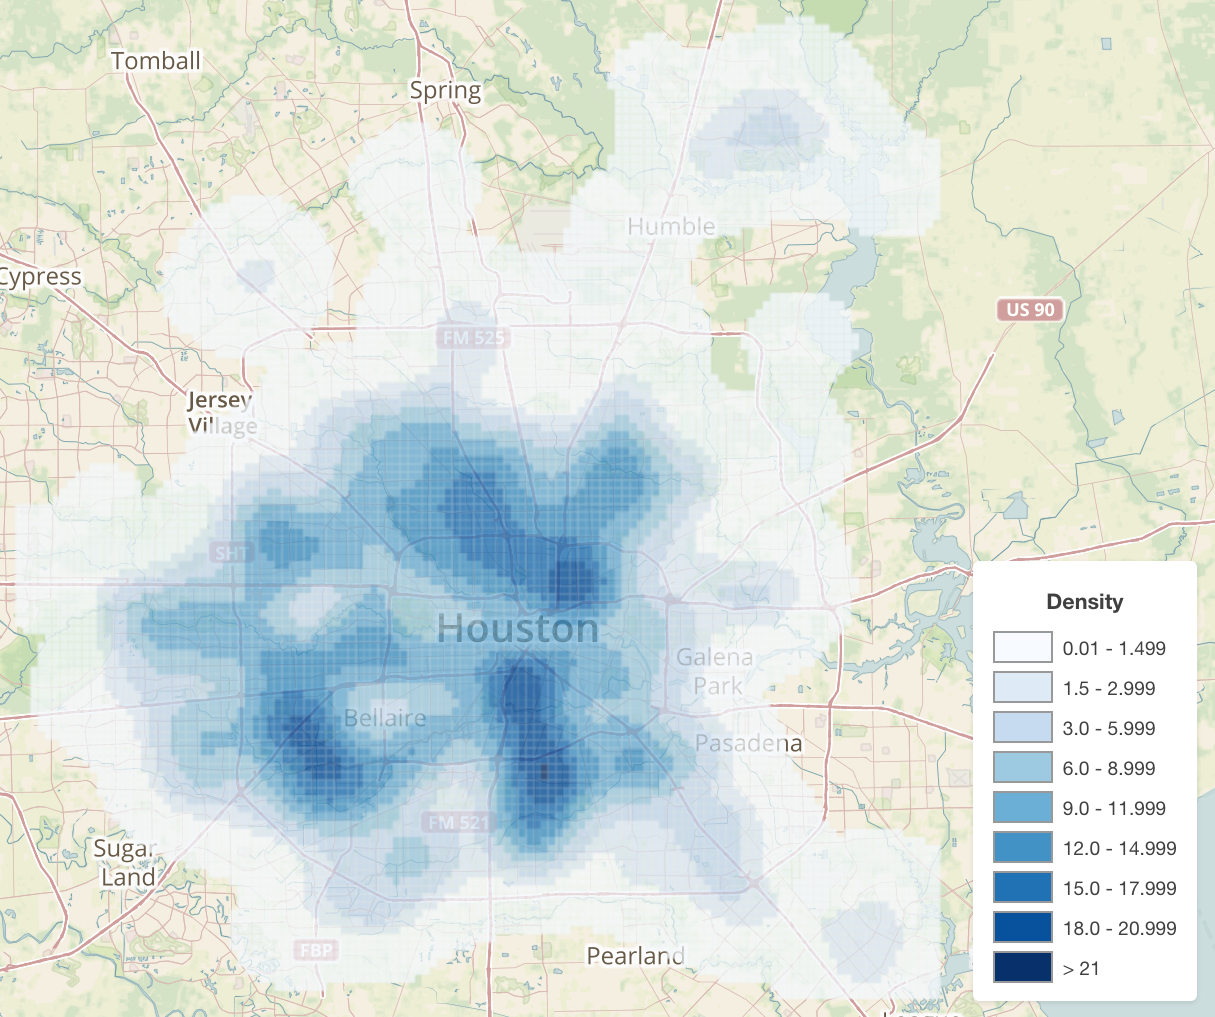
\includegraphics[width=0.7\textwidth]{./imgs/mortality_kde.png}
    \\
    b) Mortality Data
    \\
  \end{minipage}
  \caption{Kernel Density Estimates for locations of heat-related 911 calls and mortalities. 911 call data courtesy of the Houston Fire Department. Mortality data courtesy of the Texas Department of State Health Services.}
  \label{kde}
\end{figure}

Consider, for example, the two sources of data displayed in 
Figure \ref{kde}. Figure \ref{kde}a displays a kernel density estimate 
of the locations to which ambulances were dispatched in 2054 heat-related emergency calls to 911 occuring between
May and September 2006-2010 classified under at least one of the
terms ``heat,'' ``dehydration,'' ``heat exhaustion,'' or ``heat
stroke'' (exact locations of the calls cannot be shown in order
to preserve confidentiality). Figure \ref{kde}b, however, displays
a kernel density estimate of the residences of 15,244 mortalities
that occurred between May and September of the years 1999 through
2006 where the primary cause of death was connected to either
cardiovascular or kidney problems. Inevitably, some of the deaths in this group will not be directly heat-related, but both causes
have been shown to have a strong relationship with heat \citep{Kjellstrom2010}.

Examination of the kernel density estimates reveals that while the 
density of 911 calls is concentrated on a single location in the 
center of Houston, the density for the mortality data is more
diffuse, exhibiting three distinct areas of concentration. 
The fact that the spatial distribution of heat-related 911 calls
is different than that of heat-related mortalities suggests that
each measure captures only part of the overall effects of heat on
health. As a result, being able to combine the information
contained in each of the different data sources into a single risk
map in a systematic, model-based fashion becomes a useful tool
in understanding how different areas in a city are impacted 
by extreme heat as opposed to a more narrow view of where a
911 call or mortality is most likely to take place.

\subsection{Research Goals and Contributions}
Motivated by the multifaceted impact of heat on health in Houston, we seek to model multiple health outcomes jointly and create a single, combined risk map for heat across Houston, TX.  The basic tool that we employ to achieve this goal is a Poisson point process which we review briefly here; the interested reader is directed to \cite{Moller2003}, \cite{Gelfand2010}, 
or \cite{Banerjee2014} for a more rigorous treatment.  
A \textit{spatial} point process is a random process on a 
spatial domain $\mathcal{D}$ where realizations consist of a finite 
set of spatial locations $\mathcal{S} = \{\mathbf{s}_1,\dots,\mathbf{s}_n: 
\mathbf{s}_i \in \mathcal{D}\text{ }\forall\text{ } i\}$. The distribution of 
$\mathcal{S}$ is governed by an intensity function $\Lambda(\mathbf{s}): 
\mathcal{D} \rightarrow [0, \infty)$.  The point process is said to be 
Poisson because for any subset $\mathcal{B} \subseteq \mathcal{D}$,
 $N(\mathcal{B})$, the random number of points falling in $\mathcal{B}$,
is distributed $\mathcal{P}(\delta)$ where $\mathcal{P}(\delta)$ denotes
the Poisson distribution with mean $\delta = \int_{\mathcal{B}} \Lambda(\mathbf{s})d\mathbf{s}$.
Further, the density of the realized set of locations $\mathcal{S}$ is given 
by the normalized intensity
$\lambda(\mathbf{s}) = \Lambda(\mathbf{s})/\int_\mathcal{D}\Lambda(\mathbf{s})d\mathbf{s}$.   
In statistical analysis for point patterns, $\Lambda(\mathbf{s})$ is unknown.  Hence, 
focus is on parameterizing, and subsequently estimating, $\Lambda(\mathbf{s})$. 

Treating the heat-related 911 calls and mortalities as realizations of a point pattern, we seek to parameterize two unknown intensity surfaces, say $\Lambda_1(\mathbf{s})$ and $\Lambda_2(\mathbf{s})$, where each surface represents a ``risk map'' such that regions where $\Lambda_1(\mathbf{s})$ (or $\Lambda_2(\mathbf{s})$) is high are regions where a heat stress-related 911 call or mortality is likely to occur.  
Examples using point pattern models as risk maps are prevalent and include 
\cite{Best2000}, \cite{Chakraborty2011}, \cite{Heaton2014}, and 
\cite{Heaton2015} to name only a few. The inherent difficulty with point process models lies in modelling the infinite-dimensional intensity surfaces, $\Lambda_1(\mathbf{s})$ and $\Lambda_2(\mathbf{s})$.  Popular choices include a Gaussian process model for $\log(\Lambda_p(\mathbf{s}))$ (referred to as the Cox process; see \citealt{Isham:2010}) but this results in difficulties in calculating the associated likelihood due to the presence of a random integral \citep{Liang2009}.  A second option, is to make each $\Lambda_p(\mathbf{s})$ proportional to a closed-form density function (e.g.\ a normal mixture density; \citealt{Chakraborty:EtAl:2010}) but specifying a sufficiently flexible density to capture the spatial variability in the Houston data would be difficult.  Finally, a third option is to use a non-parametric density \citep{Kottas:Sanso:2007} but this presents similar computational challenges to the Cox process approach.  In this article, we use principles from the Cox process approach but use a discretized intensity surface to overcome computational issues.

The majority of point process examples in the literature
consider only a single health outcome. The primary goal of this article is to utilize information
from heat-related 911 calls and mortalities to not only estimate
risk maps from each health outcome individually, but to merge each
individual map (that is, intensity surface) into a single risk map that 
portrays the spatial distribution of the cumulative risk. In this regard, our 
work is similar to \cite{Liang2009} who model multiple types of cancer but 
do not consider merging the individual risk maps. To merge multiple intensity 
surfaces, we first model each health outcome as a 
realization of a point pattern with a specific intensity function (e.g.\ $\Lambda_1(\mathbf{s})$ and $\Lambda_2(\mathbf{s})$).  Then,
hierarchically, these individual intensity functions are treated as 
random draws from a ``cumulative'' or ``mean'' intensity function that
acts as a combined risk map for the city of Houston. By defining the
risk maps in this hierarchical modeling framework, uncertainty associated
with each intensity surface can be appropriately quantified.

Beyond the spatial distribution of the 911 calls and mortalities, it is
also of epidemiological interest to compare demographics for each heat-related
health outcome. For example, the 911 call and mortality data sources also include
the age, race/ethnicity, and gender of the respective individual. A secondary
contribution of this research is estimating the differences in demographics
among the various health outcomes. Therefore, we append the aforementioned 
point patterns also to include the intensity surfaces for the associated
marks of age, gender and race/ethnicity. This allows for a model-based comparison of 
how heat affects subpopulations differently. Because each of the associated 
marks are discrete, we introduce a modeling framework that allows for conjugate 
updates of the associated non-spatial intensity surfaces.

In summary, there are three primary contributions of this research, two statistical and one epidemiological: (i) introduction of a computationally feasible, discrete parameterization of intensity surfaces for point pattern models, (ii) development of a hierarchical framework for merging multiple risk maps, and (iii) identifying differential risks to multiple health outcomes among subpopulations. The remainder of this paper is as follows: Section 2 outlines the statistical model we use to analyze the data and to produce the desired risk maps.
Section 3 includes the generated risk maps for the 911 and mortality data
and details the results. Finally, section 4 discusses the implications
of our results and provides suggestions for future research.

\section{Statistical Model}\label{model}
This section describes a hierarchical model for merging heat-related 911 calls 
and mortalities in order to estimate a cumulative risk map. The model is presented 
in terms of (i) the likelihood layer describing the distributional assumptions 
of the observed point patterns, (ii) the process layer describing how the two health 
outcomes are interrelated and, finally, (iii) the prior layer describing 
\textit{a priori} assumptions of model parameters.

\subsection{Likelihood Layer}\label{likelayer}
Let $\mathbf{s}_{pi} \in \mathcal{D}$ be the latitude-longitude coordinate
of the location for the $i^{\text{th}}$ 
individual who experienced health outcome $p$ where $i=1,2,\dots,n_p$, $p=1,2,\dots,P$, 
such that $P$ is the total number of health outcomes under consideration (in this article, $P=2$),
and $n_p$ is the total number of individuals who experienced health outcome $p$.
Likewise, let $a_{pi} \in \left\{0,1,2,\dots,113\right\}$ represent the age of the $i^{\text{th}}$ individual who
experienced health outcome $p$; 
$g_{pi} \in \left\{\text{female}, \text{male}\right\}$ represent the gender of individual $i$ who experienced health 
outcome $p$; and $e_{pi} \in \left\{\text{Asian}, \text{Black}, \text{Hispanic}, 
\text{White}\right\}$ be the race/ethnicity of individual $i$ who experienced health
outcome $p$. The upper bound of 113 for age was chosen arbitrarily but, in our data, 
there were no individuals with an age greater than 113. For other applications, this upper 
bound may need to be adjusted to account for the possibility of older ages. 
Finally, define $\mathbf{z}_{pi} = (\mathbf{s}_{pi}',a_{pi},g_{pi},e_{pi})' \in 
\mathcal{Z}$ to be the vector of realized spatial locations and marks.

As stated in Chapter 1, we model $\{\mathbf{z}_{pi}\}_{i=1}^{n_p}$ as a
realization from a Poisson point process with unknown and nonuniform intensity surface
$\Lambda_{p}(\mathbf{s}, a, g, e)$ for $p=\left\{1, \dots, P\right\}$.  We choose to factor 
\begin{align}
\Lambda_p(\mathbf{z}) = \Lambda_p(\mathbf{s}, a, g, e) = \delta_p\alpha_p(a)\gamma_p(g)\xi_p(e)
\lambda_p(\mathbf{s})
\label{Lambda}
\end{align}
where $\delta_p$ is an unknown constant controlling the 
expected number of individuals who experience health outcome $p$; 
$\alpha_p(a)$ is the probability of an individual with health outcome 
$p$ being of age $a$; $\gamma_p(g)$ is the probability of an individual with health
outcome $p$ being of gender $g$; and $\xi_p(e)$ is the probability of an individual 
with health outcome $p$ being of ethnicity $e$. In contrast, because $\mathbf{s}$ is 
continuous, $\lambda_p(\mathbf{s})$ 
is the density at location $\mathbf{s}$ for health outcome $p$. Notably, the model in 
\eqref{Lambda} not only defines a risk map for health outcome $p$ across space 
(via $\lambda_p(\mathbf{s})$), but also does so for each of the marks age 
(via $\alpha_p(a)$), gender (via $\gamma_p(g)$) and ethnicity (via $\xi_p(e)$).

Inherent in the factorization in \eqref{Lambda} is the assumption that the marks of 
age, gender, ethnicity and spatial location are separable.  For example, \eqref{Lambda} 
assumes that the ethnicity of an individual does not impact the location of an event 
with health outcome $p$.  Given potential ethnic/racial segmentation across the city 
of Houston, this is a strong assumption.  However, we make this assumption here because 
(i) the goal of this analysis centers on spatial risk mapping for all individuals in 
Houston so as to identify the most at-risk areas of the city regardless of ethnicity, 
age, or gender and (ii) the ethnicity for the majority of individuals in the mortality 
and 911 call data are either black or white.  Hence, assuming a separate risk map for 
each ethnicity would severely diminish the amount of data available to estimate the 
risk surface for the other ethnicities.

In order to maintain the interpretations provided above, it must be the case that each 
of $\alpha_p$, $\gamma_p$, $\xi_p$ and $\lambda_p$ sum (or integrate as is the case for 
$\lambda_p$) to 1 over their respective domains. This constraint is easily 
enforced for $\alpha_p$, $\gamma_p$ and $\xi_p$ because each is discrete;  however, 
enforcing $\int_{\mathcal{D}}\lambda_p(\mathbf{s})d\mathbf{s} = 1$ in a flexible modeling 
framework is more onerous.  Rather than using an approximation as in \cite{Liang2009},
we discretize the spatial domain $\mathcal{D}$ by dividing it into 
$K=1428$ 1-km$^2$ grid cells. Using this discretization, we parameterize
 \begin{align}
 \lambda_p(\mathbf{s}) = \sum_{k=1}^K \frac{\phi_{pk}}{\left| \mathcal{G}_k \right|}
\mathds{1}\left\{\mathbf{s} \in \mathcal{G}_k\right\},
\label{lambda}
\end{align}
where $\sum_{k=1}^{K}\phi_{pk} = 1$, $\mathcal{G}_k$ is the set of locations belonging to the
$k^\text{th}$ grid cell, $\left| \mathcal{G}_k \right|$
is the area of grid cell $k$, and
$\mathds{1}\left\{\mathbf{s} \in \mathcal{G}_k\right\}$ is an indicator function. 
Standard calculations reveal that $\int_{\mathcal{D}}\lambda_p(\mathbf{s}) = 1$ provided 
that $\sum_{k=1}^K\phi_{pk} = 1$ which leads to the interpretation that
$\phi_{pk}$ is the probability that an event with health outcome $p$ occurs in grid cell 
$k$. We note that the choice of 1-km$^2$ grid cells to perform the discretization is somewhat 
arbitrary. However, a 1-km$^2$ resolution is sufficiently fine for our purposes. Additionally, 
the grid used in the discretization matches the grid cells associated with temperature 
measurements that will be used as covariates below (see section \ref{sec:temp_data}). 

As stated above, $\phi_{pk}$ can be interpreted as the probability of an event of health 
outcome $p$ occuring in grid cell $k$. Because this probability is surely largely driven 
by the population of grid cell $k$, we set $\phi_{pk} \propto E_{pk}\exp(\phi^\star_{pk})$ 
where $E_{pk}$ is a known constant representing the expected number of 
incidents of health outcome $p$ in grid cell $k$ and the normalizing constant is simply 
$\sum_{k=1}^K E_{pk}\exp(\phi_{pk}^\star)$. We use internal standardization
\citep[see][chapter 2]{Waller2004} and calculate
\begin{align}
E_{pk} &= \frac{\sum_{k=1}^K N_{pk}}{\sum_{k=1}^K \text{Pop}_k} \times \text{Pop}_k
\end{align} 
where $N_{pk}$ is the number of incidents of health outcome $p$ that occur in grid cell 
$k$ and $\text{Pop}_k$ is the population of grid cell $k$.  The parameterization 
$\phi_{pk} \propto E_{pk}\exp(\phi_{pk}^\star)$ provides an intuitive interpretation 
for $\phi_{pk}^\star$: Namely, $\phi_{pk}^\star$ denotes the log relative risk of 
grid cell $k$. When $\phi_{pk}^\star >0$ then grid cell $k$ is said to have an elevated 
risk of heat-related health outcome $p$. Likewise, when $\phi_{pk}^\star < 0$ then grid 
cell $k$ is said to have a decreased risk of heat-related health outcome $p$. 

The population data used to calculate $E_{pk}$ was taken from the 2000 census. 
Over the area covered
by our $1428$ grid cells there are $1461$ irregularly shaped census block groups. We handle
the misalignment between the block groups and our grid cells using a method outlined
by \cite{Brunsdon2015}. In this process we calculate the intersection
between grid cells and census block groups and use this to calculate the proportion of
a grid cell that lies within a block group. If a grid cell spans multiple
census block groups, the intersection will be split between those groups; if the grid cell 
is entirely contained within a block group, then the intersection will just be the grid cell 
itself. Let $\mathcal{C}_i$ represent census block group $i$ and denote the proportion
$\omega_{ki}$ as
$$\omega_{ki} = \frac{\left| \mathcal{G}_k \cap \mathcal{C}_i \right|}
  {\left|\mathcal{C}_i\right|}.$$ 
In this equation $\left| \mathcal{G}_k \cap \mathcal{C}_i \right|$ represents
the area of the intersection between grid cell $k$ and block group $i$ and 
$\left| \mathcal{C}_i \right|$ is the area of block group $i$. 
Defining $\text{CensPop}_i$ as the population count in $\mathcal{C}_i$ allows us to approximate the population count
within grid cell $k$ as $$\text{Pop}_k = \sum_{i=1}^{N} \omega_{ki}\cdot \text{CensPop}_i,$$
where $N$ is the total
number of census block groups that intersect with grid cell $k$. Therefore, population within
a given block group is distributed among intersecting grid cells based on the proportion
of the group contained within a given grid cell. One weakness of this 
method is that it assumes that the population within
a census block group is distributed equally throughout that group, which is almost
certainly not the case. Unfortunately, due to restrictions on census data, demographic information (which we use elsewhere in the model) is not available at a finer resolution. As a result, we feel this approach is justified in order to keep all census data incorporated in the model on the same scale.

\textcolor{red}{A potential solution to avoid realigning the census data to the grid cells is to let the census block groups equal the $\mathcal{G}_k$ denoted in \eqref{lambda} rather than the grid cells. However, the heat information used in this research (described in detail in Section \ref{sec:temp_data}) is provided at a 1-km$^2$ resolution and these grid cells were chosen to align exactly with the available heat data. Using the block groups in place of the grid cells would necessitate aligning the heat information to the census block group areas. Because heat is our primary variable of interest we prefer realigning the demographic information to the grid associated with the heat data as opposed to the alternative. Therefore, we proceed having aligned the population data as described.}


Now let $\mathbf{Z}_p = \{\mathbf{z}_{pi}\}_{i=1}^{n_p}$ be the collection of observations for
health outcome $p$ and let $\boldsymbol{\theta}$ denote the collection of all unknown parameters 
in \eqref{Lambda} and \eqref{lambda}.  Assuming $\mathbf{z}_{pi} \perp \mathbf{z}_{p'i'}$ for
 $p \neq p'$ conditional on the intensity surfaces (that is, independent observations),  
using the derivation in Section 8.4 of \cite{Banerjee2014}, the likelihood for the 
above parameters is
\begin{align}
f(\{\mathbf{Z}_p\} \mid \boldsymbol{\theta}) &=  \prod_{p=1}^P\left[\exp\left(-\int_\mathcal{Z}\Lambda_p
(\mathbf{z})d\mathbf{x}\right)\prod_{i=1}^{n_p}\Lambda(\mathbf{z}_{ip})\right] \notag \\
&= \prod_{p=1}^P\left[\exp\left(-\delta_p\right)\delta_p^{n_p}\prod_{i=1}^{n_p}
\alpha_p(a_{pi})\gamma_p(g_{pi})\xi_p(e_{pi})\lambda_p(\mathbf{s}_{pi})\right],
\label{likelihood}
\end{align}
where $\int_{\mathcal{Z}}\Lambda_p(\mathbf{z})d\mathbf{z} = \delta_p$ because $\alpha_p(a)$, 
$\gamma_p(g)$, $\xi_p(e)$ and $\lambda_p(\mathbf{s})$ sum (or integrate) to 1.


\subsection{Process Layer}\label{process}
At the process layer of the model, we wish to combine each of the relative risks 
$\{\phi_{pk}^\star\}$ into a single relative risk map for any heat-related health outcome. 
Let $\boldsymbol{\phi}^\star_{p} = (\phi^\star_{p1}, \dots, 
\phi^\star_{pk})'$ denote the vector of log relative risks for health outcome 
$p$ across each of the $K$ spatial grid cells.  We assume, for $p=1,\dots,P$,
\begin{align} 
\boldsymbol{\phi}_p^\star \overset{ind}{\sim} \mathcal{N}\left(\boldsymbol\mu, \sigma^2_p\mathbf{M}_p\right),
\label{phiprior}
\end{align}
where $\boldsymbol{\mu} = (\mu_1,\dots,\mu_K)'$ is the mean vector of log relative risks
across all $P$ health outcomes, $\sigma^2_p$ is the variance of health outcome 
$p$, and $\mathbf{M}_p$ is the covariance matrix arising from the Mat\`{e}rn covariance 
function with smoothness parameter $\nu_p$ and decay parameter $\psi_p$. In other 
words, the $i,j$ element of $\mathbf{M}_p$ is given by $M_{\nu_p}(\|\mathbf{s}_i^\star - 
\mathbf{s}_j^\star\| \mid \psi_p)$ where $\mathbf{s}^\star_i$ is the centroid of the $i^{th}$ 
grid cell and $M(\cdot)$ is the Mat\'{e}rn covariance function.  We note, here, that 
the traditional tool for enforcing spatial correlation among areal units (grid cells) 
is the conditional autoregressive (CAR) model; however, the CAR model is defined in terms 
of pairwise differences and is, hence, not ``centered.''  Because we wish to estimate 
the mean of multiple log relative risks, we opt for the Mat\'{e}rn covariance model to 
enforce spatial correlation.

The vector $\boldsymbol\mu$ is of particular interest in our model because it represents
the combination of information from many different sources of health data into
a single measure of the overall relative risk of heat on 
health rather than just the impact of heat on one indicator. In spite of a common mean, 
in \eqref{phiprior} we allow a separate variance parameter for each health outcome 
($\sigma^2_p$). We make this assumption primarily from the kernel density estimates 
in Figure \ref{kde} which 
show that the density of the 911 calls is more peaked (i.e. larger variance of density values).

An implicit assumption with \eqref{phiprior} is the independence assumption among the log relative risks for each health outcome given the overall, ``cumulative'' log relative risk surface $\boldsymbol{\mu}$. For the application considered here this assumption is likely to, approximately, hold because the time frame for the 911 call data is 2006-2010 while the time frame for the mortality data is 1999-2006 (a minimal overlap); however, in other applications independence may not hold. In such cases, a multivariate spatial model (see \cite{Genton2015} for a discussion) could be used in place of \eqref{phiprior}. We note the possible benefit of modeling dependence between the log relative risks but we do not explore this option here.

Additionally, at the process layer of the model we assume 
\begin{align}
\boldsymbol{\mu} \sim \mathcal{N}(\mathbf{X}\boldsymbol{\beta},\sigma^2_\mu\mathbf{M}_\mu)
\label{mu}
\end{align}
where $\mathbf{X}$ is a $K\times Q$ design matrix of covariates with associated coefficients 
$\boldsymbol{\beta}$, $\sigma^2_\mu$ is a variance and $\mathbf{M}_\mu$ is a spatial correlation 
matrix implied by the Mat\'{e}rn correlation function with smoothness $\nu_\mu$ and 
decay $\psi_\mu$. The regression in \eqref{mu} allows us to assess if covariates such as 
poverty, age, or urban temperature affect the height of the global intensity surface 
through inference on the parameters $\boldsymbol{\beta}$.

\subsection{Hyperprior Layer}
\textcolor{red}{At the hyperior prior layer of the model, we outline our prior assumptions for the model
parameters in Sections \ref{likelayer} and \ref{process}. Because $\boldsymbol{\alpha}_p = 
(\alpha_p(0),\dots,\alpha_p(113))'$ are probabilities where $\sum_a \alpha_p(a) = 1$, 
we assume $$\boldsymbol{\alpha}_{p} \sim \text{Dir}(\mathbf{1}_{113})$$ for all $p$ where 
$\text{Dir}(\cdot)$ denotes the Dirichlet distribution and $\mathbf{1}_{113}$ is a $1\times 113$ vector of ones. Note that for a symmetric Dirichlet distribution with a concentration parameter of 1 across $M$ categories, its density function simplifies to 
\begin{equation}
\frac{1}{C}\prod_{i=1}^M x_i^{1 - 1} = \frac{1}{C},
\end{equation}
where $C$ is a constant. Therefore, assuming $\boldsymbol\alpha_p \sim \text{Dir}(\mathbf{1}_{113})$ is equivalent to applying a uniform prior to $\boldsymbol\alpha_p$, and it follows that it is non-informative. Further, if we let $f(\boldsymbol\alpha_p)$ and $f(\boldsymbol\alpha_p \mid \mathbf{Z}_p)$ represent the prior and posterior distributions for $\alpha_p$, respectively, and let $n_{p,a}$ be the number of people who experienced health outcome $p$ at age $a$, then we can use the likelihood in \eqref{likelihood} to show that the Dirichlet prior described for $\boldsymbol{\alpha}_p$ is conjugate:  
\begin{align}
f(\boldsymbol{\alpha}_p \mid \mathbf{Z}_p) &\propto \text{f}(\boldsymbol{\alpha}_p)f(\mathbf{Z}_p \mid \boldsymbol\Theta) \notag \\
&\propto \left[\prod_{a=0}^{113}\left(\alpha_p(a)\right)^{1-1}\right]\left[\prod_{a=0}^{113} \left(\alpha_p(a)\right)^{n_{p,a}}\right]  \label{apost} \\
&= \prod_{a=0}^{113} \left(\alpha_p(a)\right)^{(n_{p,a}+1)-1}. \notag
\end{align} 
Stated explicitly, the posterior distribution of $\boldsymbol\alpha_p$ is a Dirichlet distribution with concentration parameters $(n_{p,0} + 1, n_{p,1} + 1, \dots, n_{p,113}+1)$.
In a similar vein, we assume $$\boldsymbol\gamma_p = (\gamma_p(\text{female}), \gamma_p(\text{male}))' \sim \text{Dir}(\mathbf{1}_2)$$ and $$\boldsymbol\xi_p = (\xi_p(\text{Asian}), \dots, \xi_p(\text{White}))' \sim \text{Dir}(\mathbf{1}_4),$$ which, by the same argument, are also non-informative and conjugate priors.}


\textcolor{red}{Our approach for the remaining unknown parameters is to assume vague priors (and conjugate 
where possible). %Is the following sentence sufficient to explain why we use vague priors?
This is justified because there is sufficient data to learn these parameters without the need to rely heavily on prior information. For $\delta_p$, we assume $\delta_p \sim \mathcal{G}(0.001, 0.001)$, where $\mathcal{G}(a,b)$ denotes the gamma distribution with shape $a$ and rate $b$. Note that for $\delta_p$ the likelihood in \eqref{likelihood} is proportional to $$\exp\left(-\delta_p\right)\delta_p^{n_p},$$ the kernel of a Poisson distribution. Therefore, the gamma prior for $\delta_p$ is conjugate, producing a posterior distribution of $\mathcal{G}(n_p + 0.001, 1 + 0.001)$. We assume $\{\sigma^2_p\}$ and $\sigma^2_\mu$ are independent 
$\mathcal{IG}\left(2.001, 1.001\right)$ 
random variables where $\mathcal{IG}(a,b)$ denotes the inverse-gamma distribution with scale 
$a$ and rate $b$, a well-known conjugate prior for normal variance parameters. The $\mathcal{IG}(2.001, 1.001)$ distribution has a variance of 1000, providing sufficient flexibility for the data to accurately dictate the variances. For the regression coefficients we assume that $\boldsymbol{\beta} \sim 
\mathcal{N}(0, 50\mathbf{I}_{Q})$, leading to a Gaussian complete conditional for $\boldsymbol{\beta}$. 
Conjugate prior distributions for each spatial smoothness parameter (the $\nu$'s) and decay 
parameter (the $\psi$'s) are not available; however, following the results of \cite{Zhang2004}, 
a vague prior for the variance parameters (the $\sigma^2$'s) allows each smoothness and decay 
parameter to be fixed without loss generality or predictive power.}

\subsection{Model Fitting}
\textcolor{red}{We fit this model within a Bayesian framework. For each health outcome $p = 1, \dots, P$, randomly generate draws for $\delta_p$ from the known posterior, $\mathcal{G}(n_p + 0.001, 1.001)$. Similarly, because the priors
for $\boldsymbol{\alpha}_p$, $\boldsymbol{\gamma}_p$, and $\boldsymbol{\xi}_p$ are all conjugate, their posterior
distributions are known and can be drawn from directly. That is, we can easily obtain random draws from $\text{Dir}(n_{p,0} + 1, n_{p,1} + 1, \dots, n_{p,113})$, $\text{Dir}(n_{p,Female} + 1, n_{p,Male} + 1)$, and $\text{Dir}(n_{p,Asian} + 1, \dots, n_{p,White} + 1)$, where as before $n_{p,0}$ denotes the number of people who experienced health outcome $p$ at age $0$, $n_{p,Female}$ indicates the number of females who experienced health outcome $p$, and so on.}

 \textcolor{red}{The posterior densities for the rest of the parameters are unknown and so we obtain draws from the posterior using a Metropolis within Gibbs sampler of the following form:
\begin{enumerate}
  \item \label{draws2} For $p = 1, \dots, P$, sample $\sigma^2_p \sim \mathcal{IG}(2.001 + \frac{K}{2}, 1.001 + \frac{1}{2}\boldsymbol\phi^{\star\prime}\mathbf{M}_p^{-1}\boldsymbol\phi^\star)$;%[ \sigma^2_p | \boldsymbol{\phi}^\star_p, \mathbf{M}_p]$;
  \item \label{drawphi} For $p = 1, \dots, P$, sample $\boldsymbol\phi^\star_p \sim [ \boldsymbol\phi^\star_p | \sigma^2_p, \mathbf{M}_p ]$;
  \item \label{drawsmu} Sample $\sigma^2_\mu \sim \mathcal{IG}(2.001 + \frac{K}{2}, 1.001 + \frac{1}{2}(\boldsymbol\mu - \mathbf{X}\boldsymbol\beta)^\prime\mathbf{M}^{-1}_\mu(\boldsymbol\mu - \mathbf{X}\boldsymbol\beta));$%[ \sigma^2_\mu | \boldsymbol{\mu}, \boldsymbol{\beta}, \mathbf{M}_\mu ]$;
  \item \label{drawmu} Sample $\boldsymbol{\mu} \sim [ \boldsymbol{\mu} | \{\boldsymbol{\phi}^\star_p\}, 
    \{\sigma^2_p\}, \{\mathbf{M}_p\}, \sigma^2_\mu, \mathbf{M}_\mu, \boldsymbol{\beta} ]$; and
  \item \label{drawbeta} Sample $\boldsymbol{\beta} \sim \mathcal{N}(\sigma_\mu^{-2}\Sigma^{\star}\mathbf{X}^\prime\mathbf{M}_\mu^{-1}\boldsymbol\mu, \Sigma^\star)$, where $\Sigma^\star = \left[\frac{1}{50}I_Q + \frac{1}{\sigma^2_\mu}\mathbf{X}^\prime \mathbf{M}_\mu^{-1}\mathbf{X}\right]^{-1}$.%[ \boldsymbol{\beta} | \boldsymbol{\mu}, \sigma^2_\mu, \mathbf{M}_\mu ]$.
\end{enumerate}}

Note that for steps \ref{draws2}, \ref{drawsmu}, and \ref{drawbeta} we have the complete conditional distributions, but that \ref{drawphi} and \ref{drawmu} require a Metropolis-Hastings (MH) update. Using a sampler of this design, 10000 draws were taken from the posterior distributions for each of these parameters, after a burn-in of 10000. Monte Carlo standard error (MCSE) was calculated for each chain and provided evidence that all of them converged \citep{Flegal2015}. 


\section{Results}\label{results}
%For sake of clarity, throughout this section we will let $p =1$ denote the 911 calls and $p=2$ denote the heat-related mortalities.

\subsection{Covariates and Variable Selection}\label{sec:temp_data}
Recall that in \eqref{mu} we regressed $\boldsymbol{\mu}$ on covariates $\mathbf{X}$ in order to account for potential confounding effects within each grid cell.   For this analysis, the $\mathbf{X}$ matrix denoted above consists of an intercept, temperature data defined below, the percent of people over 65 in each grid cell and the number of people without central air conditioning in a given grid cell. Percent of people over 65 was taken from 2010 U.S. Census Data and the number of people without air conditioning was taken from the Harris County tax assessor parcel database. Both were aligned with our discrete grid using the method described in Section \ref{likelayer}. 

In order to get heat information at the resolution necessary for this
study, we used temperature data simulated using an offline version of the 
Noah Land Surface Model, known as the High Resolution Land Data Assimilation 
System (HRLDAS).
These data consist of 15,625 HRLDAS 1-km$^2$ grid boxes that cover the Houston
area and contain 6 temperature measurements that we consider: daily max/min 
temperature at 2 meters above the ground (T2), daily max/min NWS heat index (HI), and
daily max/min Swedish wet-bulb-globe temperature (SWBG). To get a measure of the 
``heat'' associated with locations across the city, the values for each of 
these variables were averaged across the months May through September of 
1999 -- 2010 (the time window for all observed health outcomes). 

We fit the model in Chapter \ref{model} using each of these temperature variables (one at a time) and then calculated the deviance information criterion (DIC) \citep{Spiegelhalter2002} as a measure of model fit. 
Table 1%\ref{DIC} 
shows that the model produced the lowest DIC value when fit with max HI so the numerical estimates and risk maps shown in this chapter are from the model fit with this temperature measurement. Figure \ref{fig:temp} displays the average maximum HI values associated with each grid cell and shows a clear spatial distribution, with higher temperatures concentrated near the city center. Note that the DIC values in Table 1
%\ref{DIC} 
are all very close, indicating little difference in model fit between the different variables.  This is, perhaps, due to the fact that the covariates enter our model at the mean intensity surface layer (in the regression for $\boldsymbol{\mu}$) at which point it is difficult to distinguish between the different heat variables. That is, because $\boldsymbol{\mu}$ captures both the 911 calls and mortalities, it is possible that any of the measured heat variables explain the combined impact of heat on ``health'' whereas specific heat variables better explain specific health outcomes.

% Table created by stargazer v.5.2 by Marek Hlavac, Harvard University. E-mail: hlavac at fas.harvard.edu
% Date and time: Tue, Nov 03, 2015 - 15:11:28
\begin{table}%\centering 
  \caption{DIC Values for Models Fit Using Each Temperature Measurement.} 
  \label{DIC} 
\begin{tabular}{@{\extracolsep{5pt}} cc} 
\\[-1.8ex]\hline
\hline \\[-1.8ex]  
Temperature Measurement & DIC \\
\hline \\[-1.8ex]  
HI Max & $220991.6$ \\ 
HI Min & $221016.2$ \\ 
T2 Max & $220998.3$ \\ 
T2 Min & $220999.9$ \\ 
SWBG Max & $221008.0$ \\ 
SWBG Min & $221021.4$ \\ 
\hline \\[-1.8ex] 
\end{tabular} 
\end{table} 


\begin{figure}
  \centering
  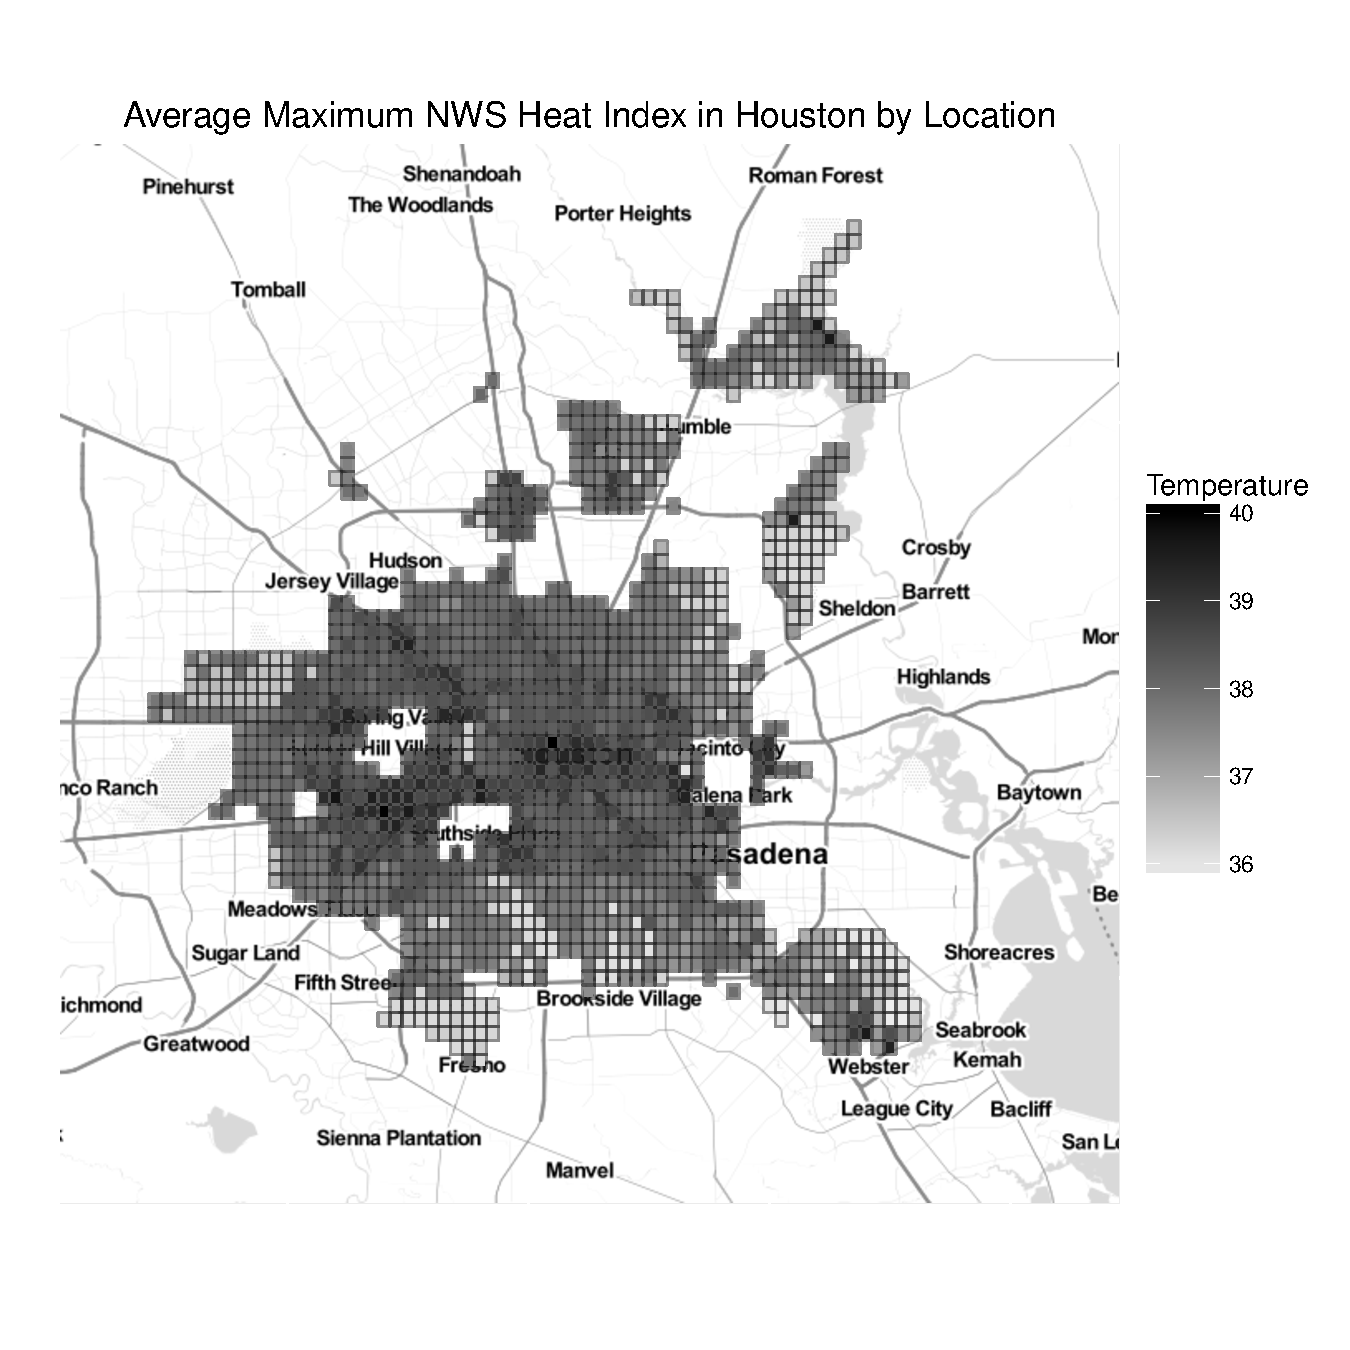
\includegraphics[width=0.7\textwidth]{imgs/avg_temp.pdf}
  \caption{Maximum NWS Heat Index in Houston, averaged over the summer months of 1999 -- 2010. Notice that there is a clear concentration of higher temperatures in the center of the city.}
  \label{fig:temp}
\end{figure}

\subsection{Risk Maps}
The maps in Figure \ref{relative_risks} show the posterior estimates for $\boldsymbol\phi^\star_{p}$ where $p\in \{911,\text{Mort}\}$, the log relative risks for each health outcome, and $\boldsymbol\mu$, the vector of log relative risks averaged across all health outcomes. Notice that in Figure \ref{relative_risks}a, the map showing $\boldsymbol\phi^\star_{911}$, the majority of the high risk area is concentrated in the city center. This is in line with the temperature measurements depicted in Figure \ref{fig:temp}, which shows a concentration of higher temperatures in the middle of Houston. Additionally, the area of highest concentration occurs in a downtown location with several parks and other walkable destinations, which may be a potential explanation for why heat-related 911 calls occur with relatively high frequency in this area. 

There is a somewhat surprising area of extremely high relative risk for 911 calls in the northern part of the city; however, inspection of the underlying geography reveals that much of this area is covered by an airport, resulting in extremely low population levels (fewer than 25 people per square kilometer) yet a relatively large incidence of heat-related 911 calls (4, 6, and 7 phone calls in each of the three affected grid cells, respectively). Another important feature of the 911 call map is that the range for $\boldsymbol\phi^\star_{911}$ is much larger than the range for either $\boldsymbol\phi^\star_{\text{Mort}}$ or $\boldsymbol\mu$ and that far more of the $\boldsymbol\phi^\star_{911}$ values reach into the upper end of the distribution, with 7.4 percent of $\boldsymbol\phi^\star_{911}$ values greater than 1, compared to just 1.2 percent of the elements of $\boldsymbol\phi^\star_{\text{Mort}}$ greater than 1 and less than 1 percent of the elements of $\boldsymbol\mu$ greater than 1. This is likely due to sparsity of data: if more heat-related 911 calls were observed, the associated locations could potentially be more diffuse than those currently observed, leading to lower relative risk scores. Notice also that the credible interval widths (see Figure \ref{relative_risks}b), unsurprisingly, are largest where no 911 calls were observed and estimation of $\phi^\star_{911,k}$ was dependent entirely on spatial correlation. 

The risk map depicting $\boldsymbol\phi^\star_{\text{Mort}}$ shown in Figure \ref{relative_risks}c also displays a concentration of high relative risk in the city center, but additionally shows a clear ``Y''-shaped pattern extending from the middle of the city. Reasons for this difference in distribution are not immediately clear, although it is worth noting that the pattern roughly coincides with several arterial thoroughfares. This demonstrates a clear difference in the spatial distribution of heat-related mortalities when compared to the spatial distribution of the 911 calls. Due to the profusion of mortality data, the associated credible interval widths are much narrower than those for the 911 call data, although many of the intervals near the city periphery are still quite large.

Figure \ref{relative_risks}e shows the spatial distribution of $\boldsymbol\mu$ and again we see heavy concentration in the center of Houston. Notice that this surface appears to be much smoother than the other two and that the range of values is compressed in comparison to both of the other health outcomes, but that in general, the areas of higher relative risk for $\boldsymbol\mu$ reflect those seen in the other two maps. Examination of the correlations between the three relative risk surfaces showed that $\boldsymbol\mu$ was correlated most highly with $\boldsymbol\phi^\star_{\text{Mort}}$ $(r=0.82)$, and that the correlation with $\boldsymbol\phi^\star_{911}$, while still strong, was slightly lower $(r=0.68)$. In both cases, the correlation between $\boldsymbol\mu$ and each $\boldsymbol\phi^\star_p$ was much stronger than the correlation between $\boldsymbol\phi^\star_{911}$ and $\boldsymbol\phi^\star_{\text{Mort}}$ $(r=0.54)$, suggesting that this mean surface is successfully borrowing information from both data sources, and that although the mortality data might carry more weight (as there are far more observations), the phone call data is still providing valuable input in the estimation of $\boldsymbol\mu$. 


\begin{figure}
  \begin{minipage}[t]{0.48\textwidth}
    \centering
    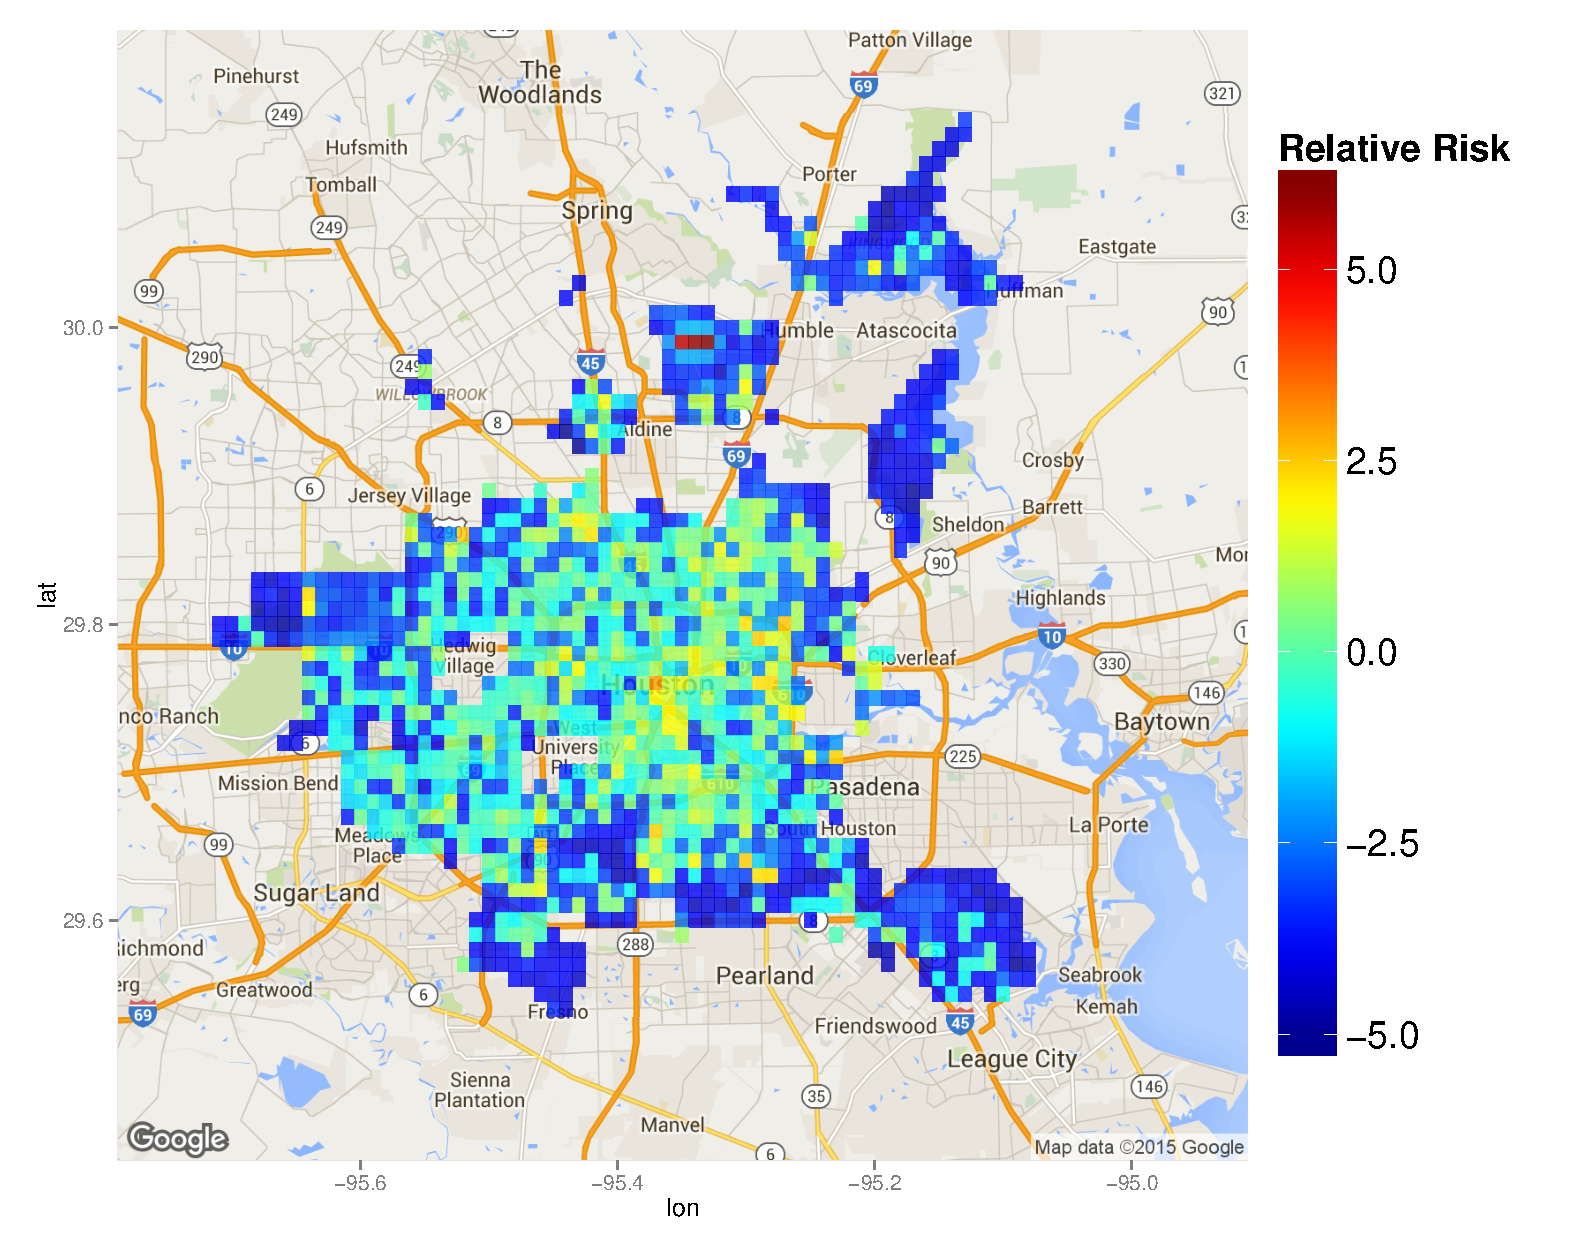
\includegraphics[width=1.0\textwidth]{./imgs/911calls_rr.pdf}
    \\
    a) 911 Data
    \\
    % rr-911
  \end{minipage}
  \hfill
  \begin{minipage}[t]{0.48\textwidth}
    \centering
    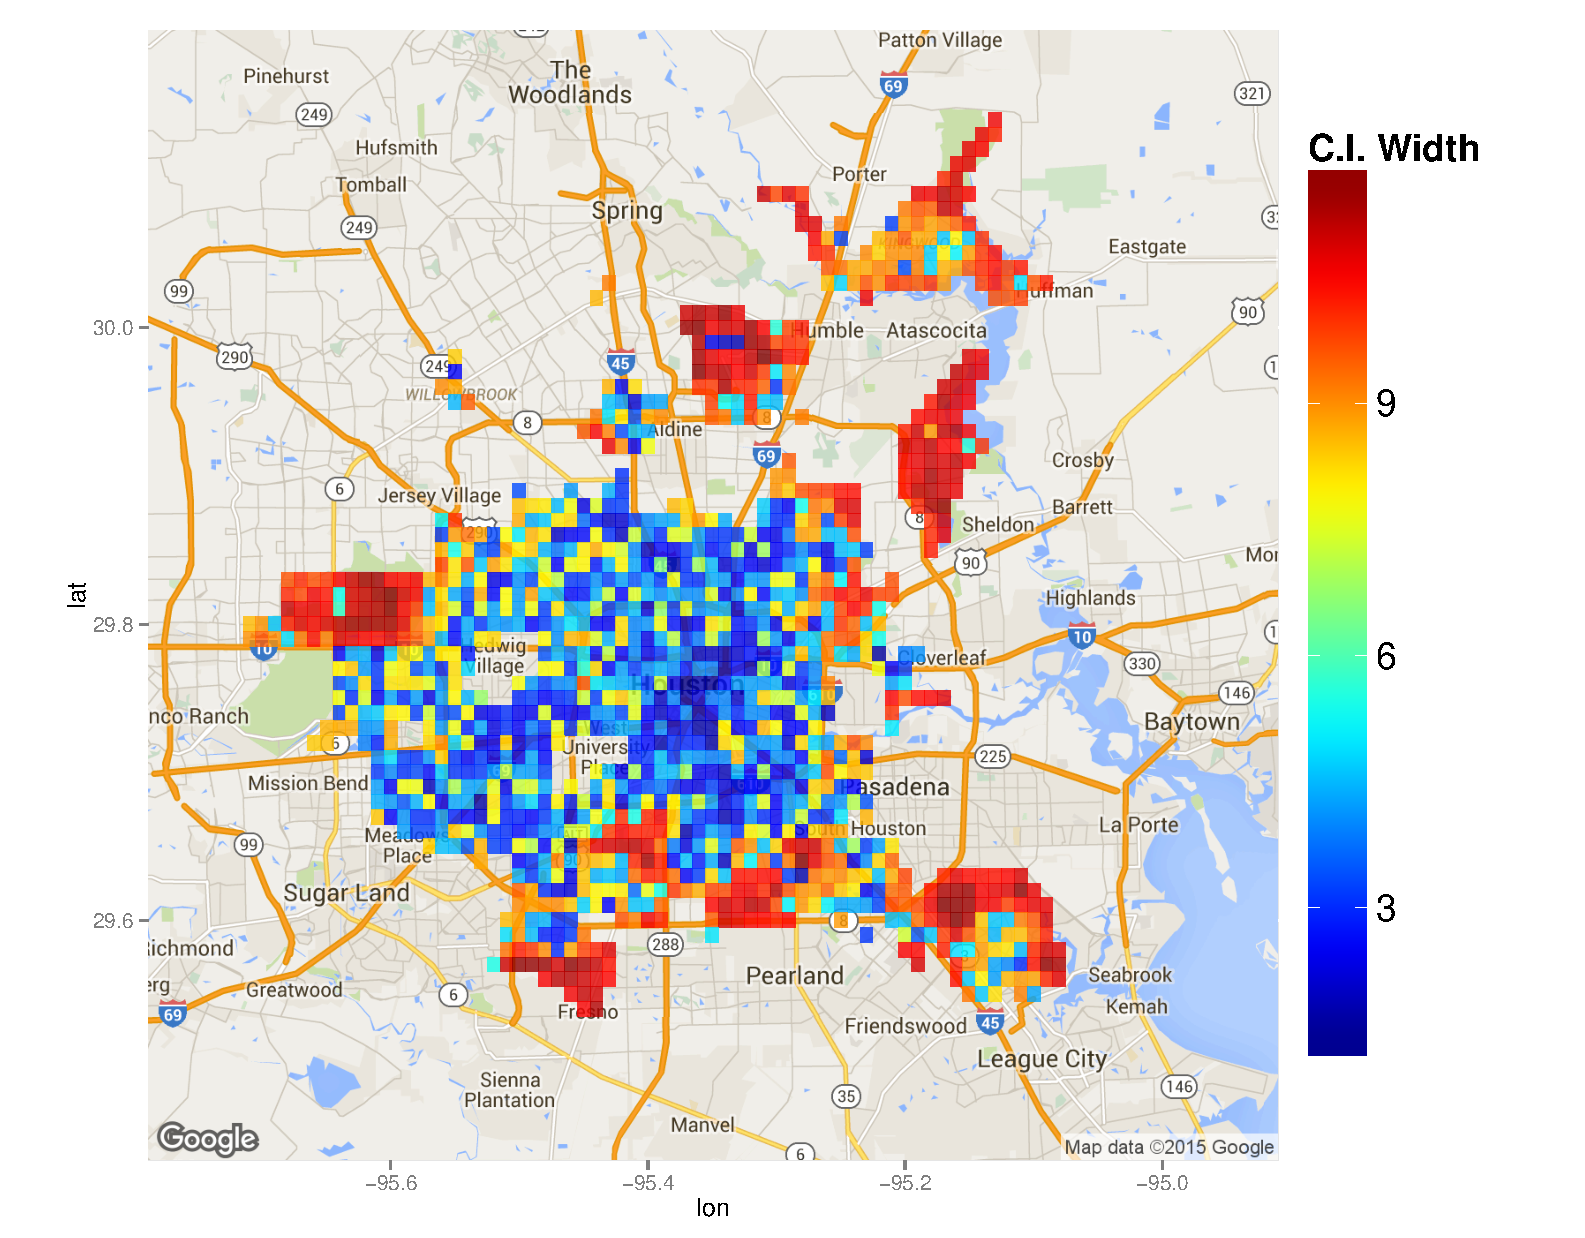
\includegraphics[width=1.0\textwidth]{imgs/911calls_ciwidths.pdf}
    \\
    b) 95\% CI Widths for 911 Data
    \\
%     \label{rr-911-ci}
  \end{minipage}
  \begin{minipage}[t]{0.48\textwidth}
    \centering
    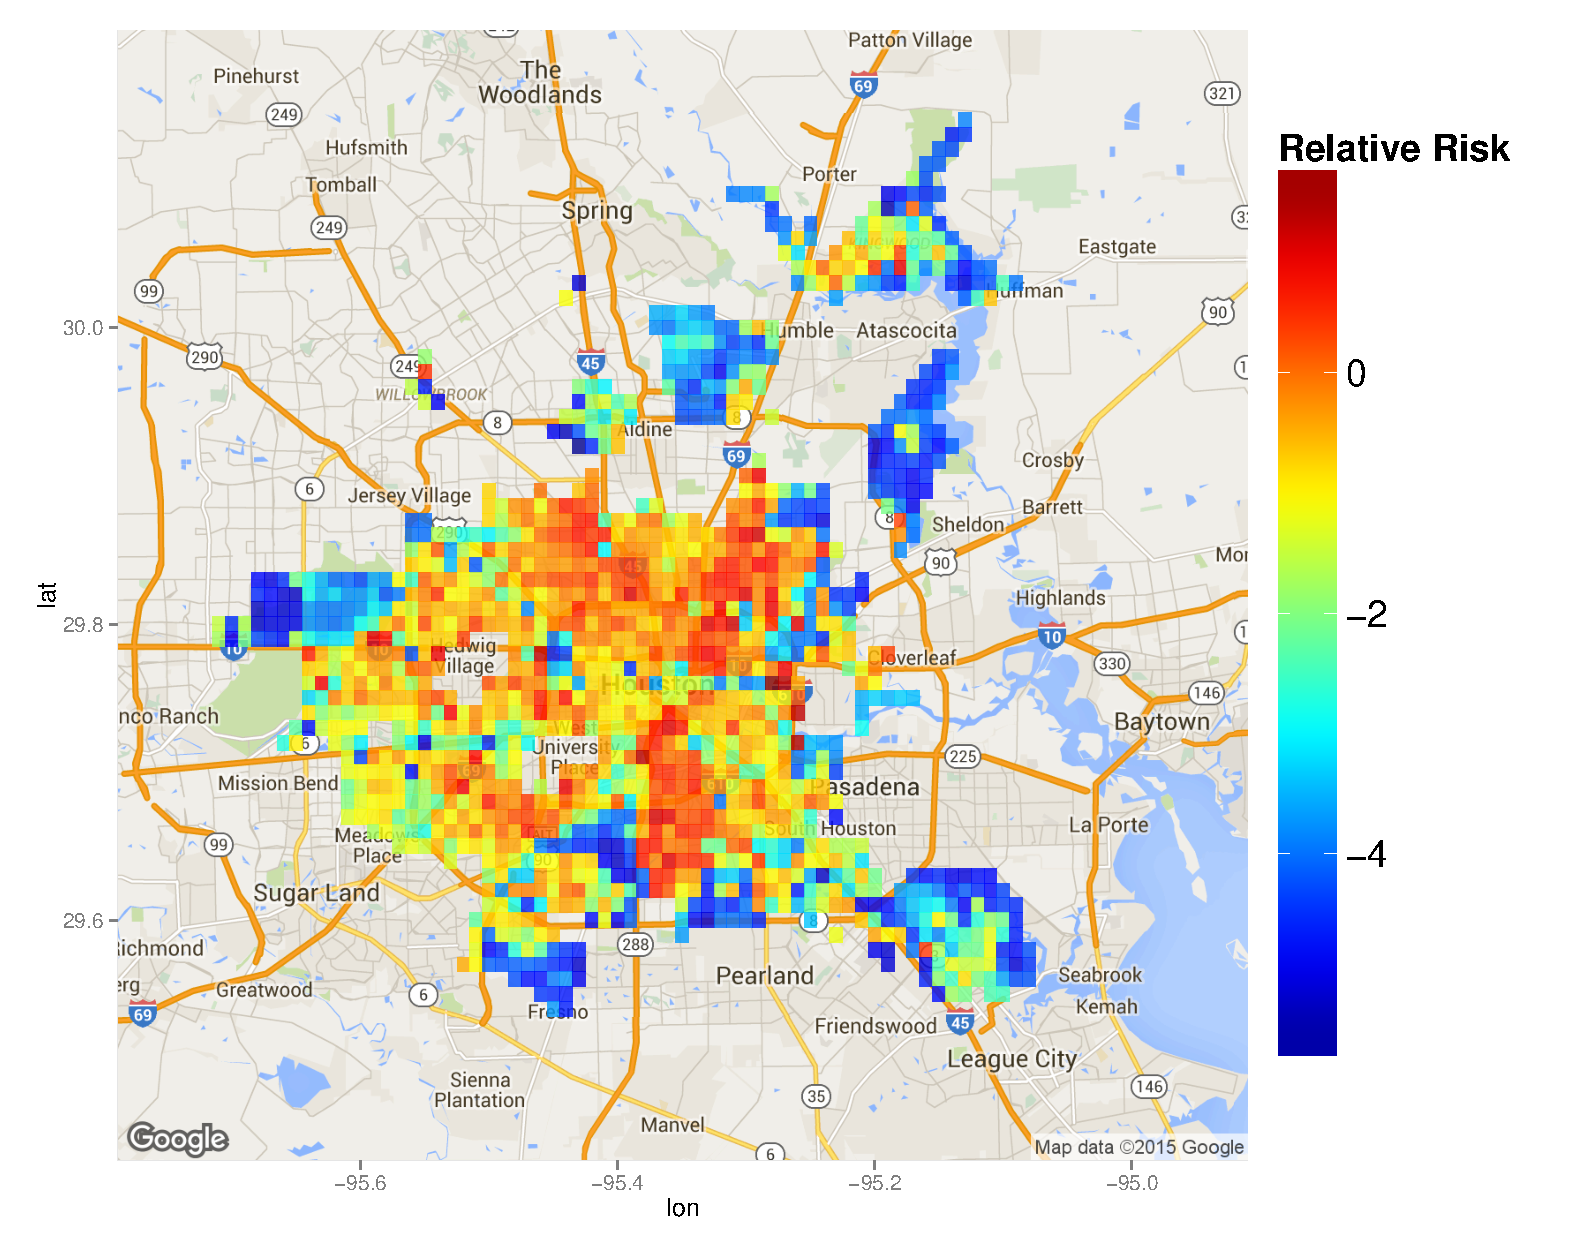
\includegraphics[width=1.0\textwidth]{./imgs/mortality_rr.pdf}
    c) Mortality Data
%     \label{rr-mort}
  \end{minipage}
  \hfill
    \begin{minipage}[t]{0.48\textwidth}
    \centering
    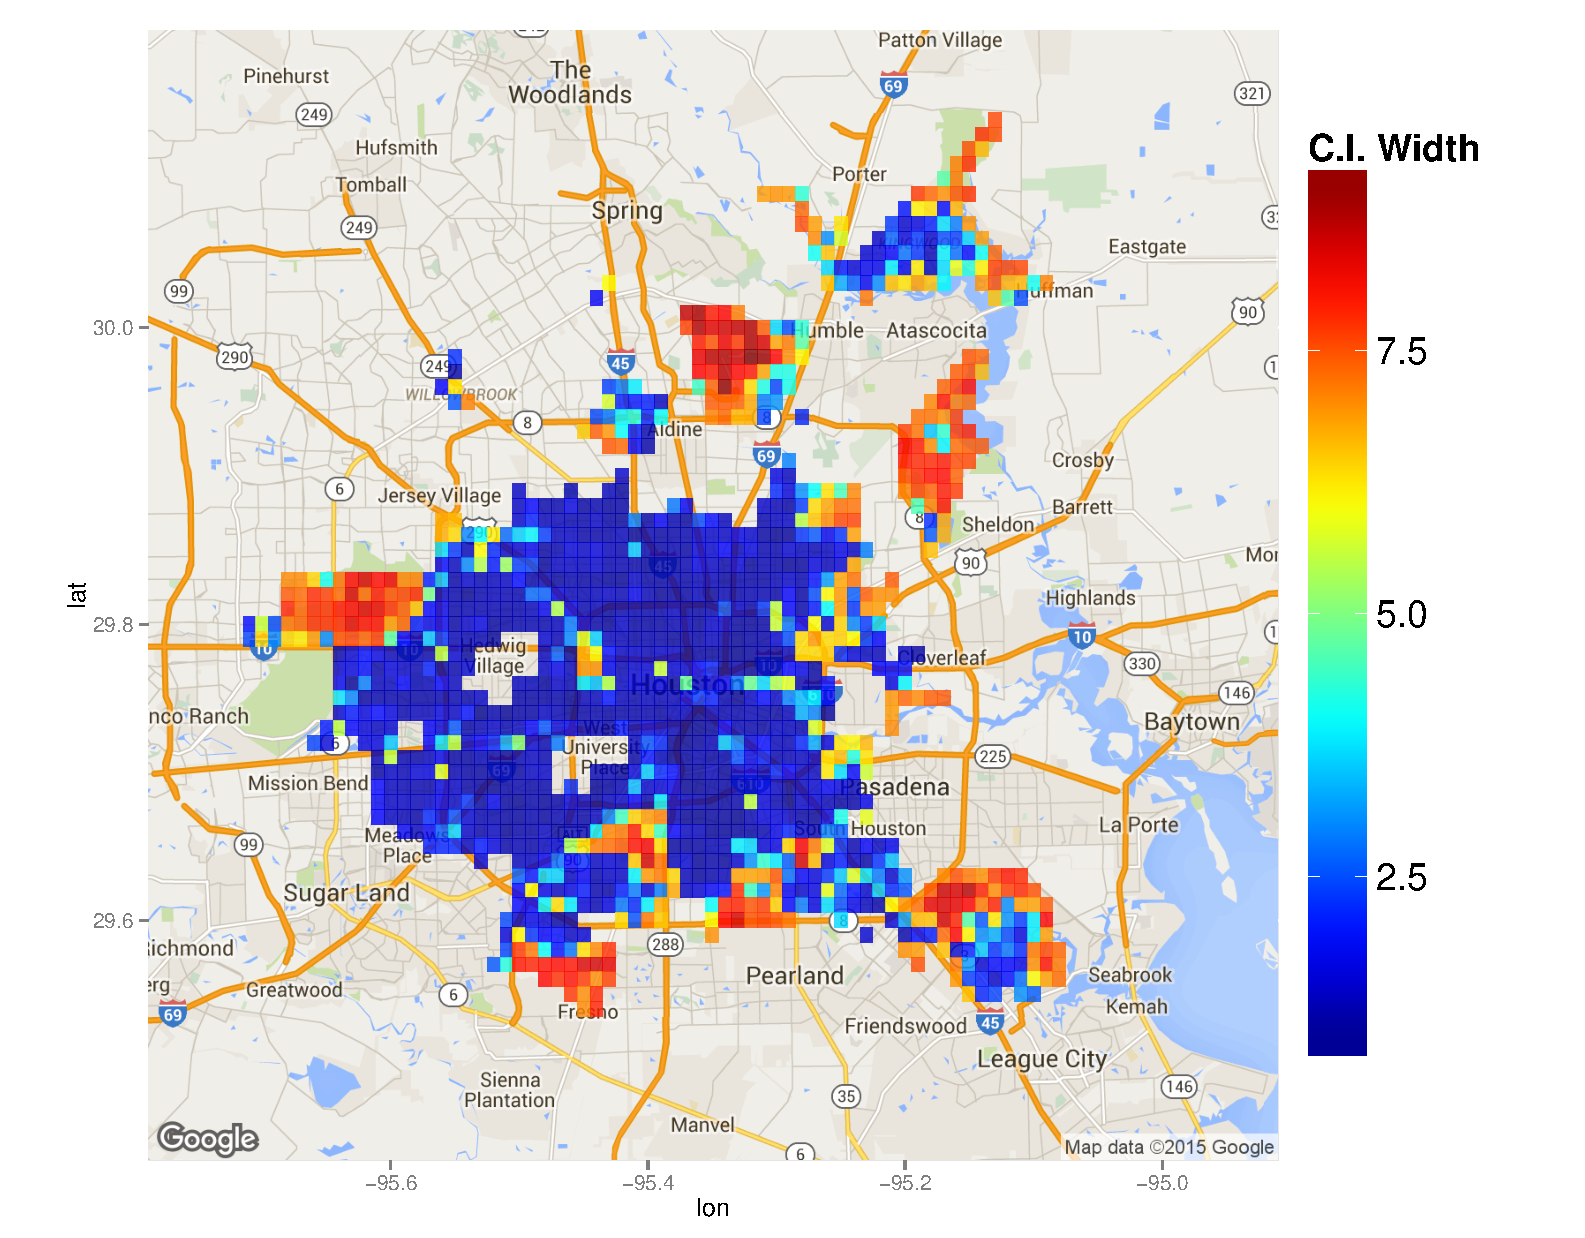
\includegraphics[width=1.0\textwidth]{imgs/mortality_ciwidths.pdf}
    d) 95\% CI Widths for Mortality Data
%     \label{rr-mortality-ci}
  \end{minipage}
  \begin{minipage}[t]{0.48\textwidth}
    \centering
    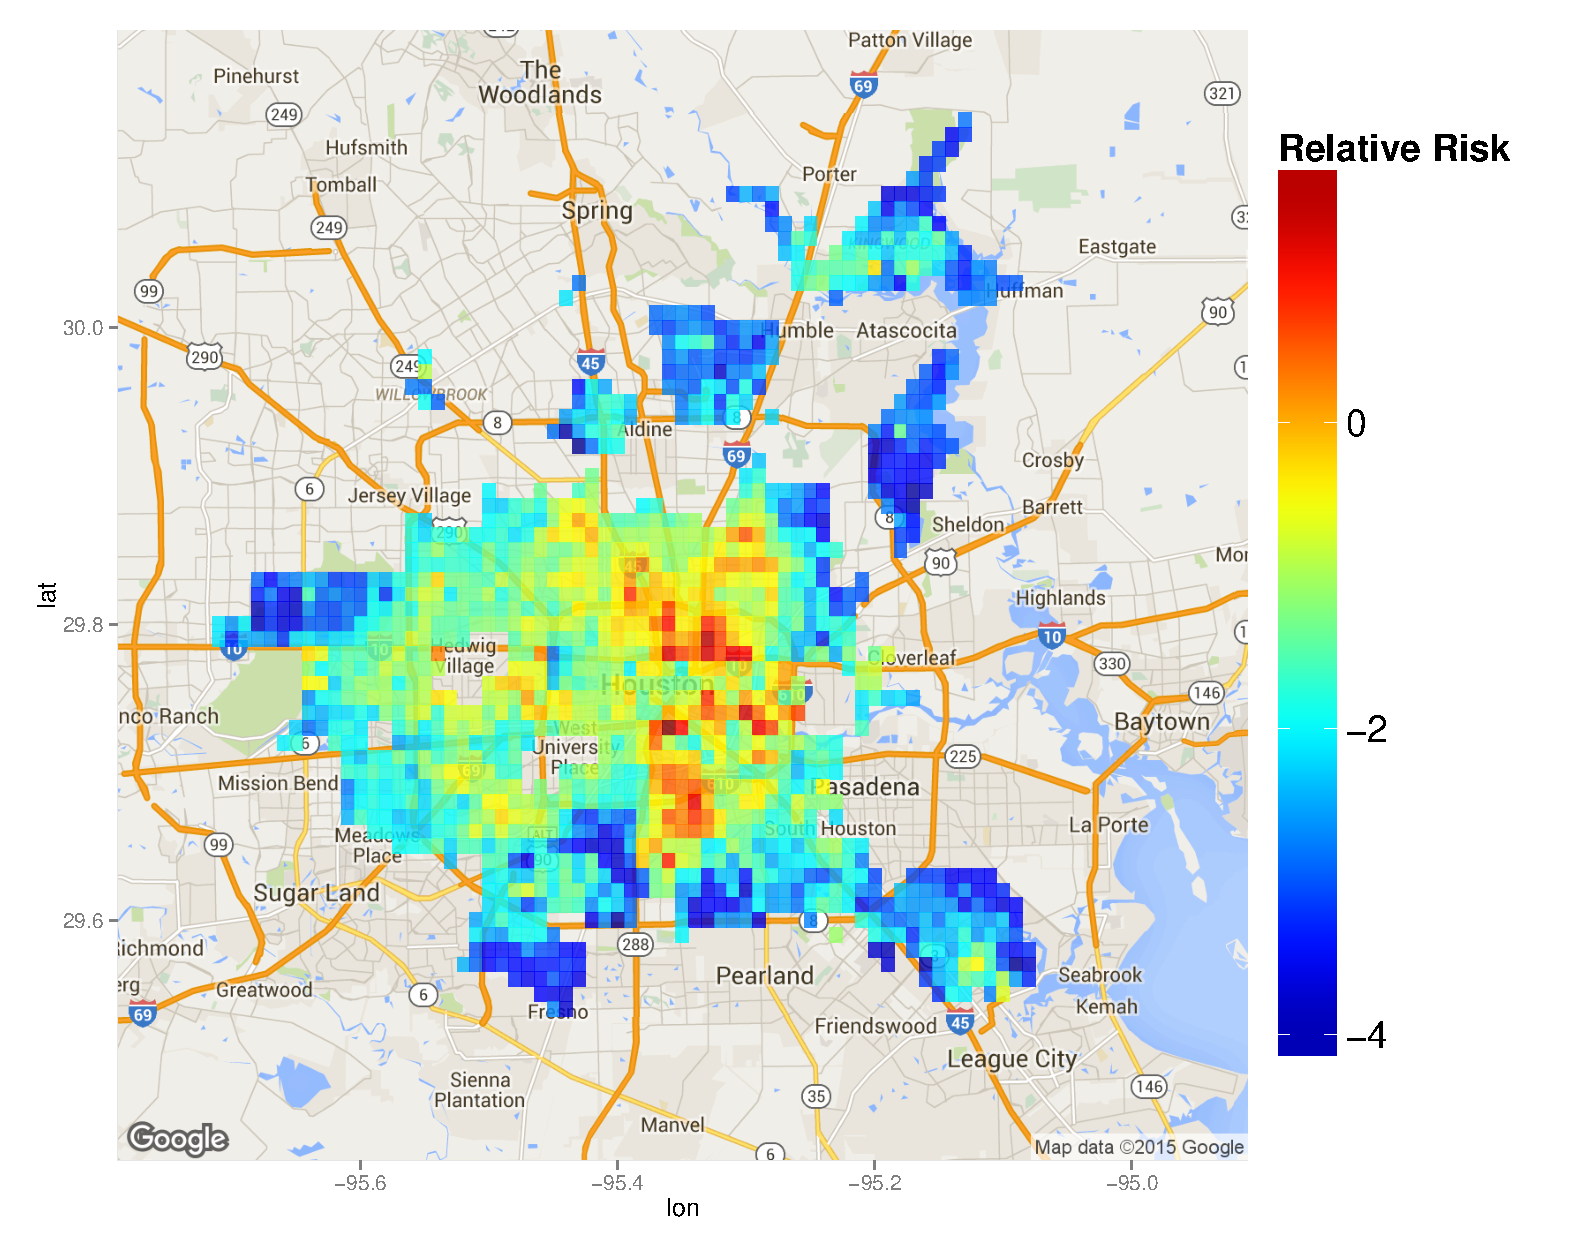
\includegraphics[width=1.0\textwidth]{./imgs/overall_rr.pdf}
    e) Overall
%     \label{rr-overall}
  \end{minipage}
  \hfill
  \begin{minipage}[t]{0.48\textwidth}
    \centering
    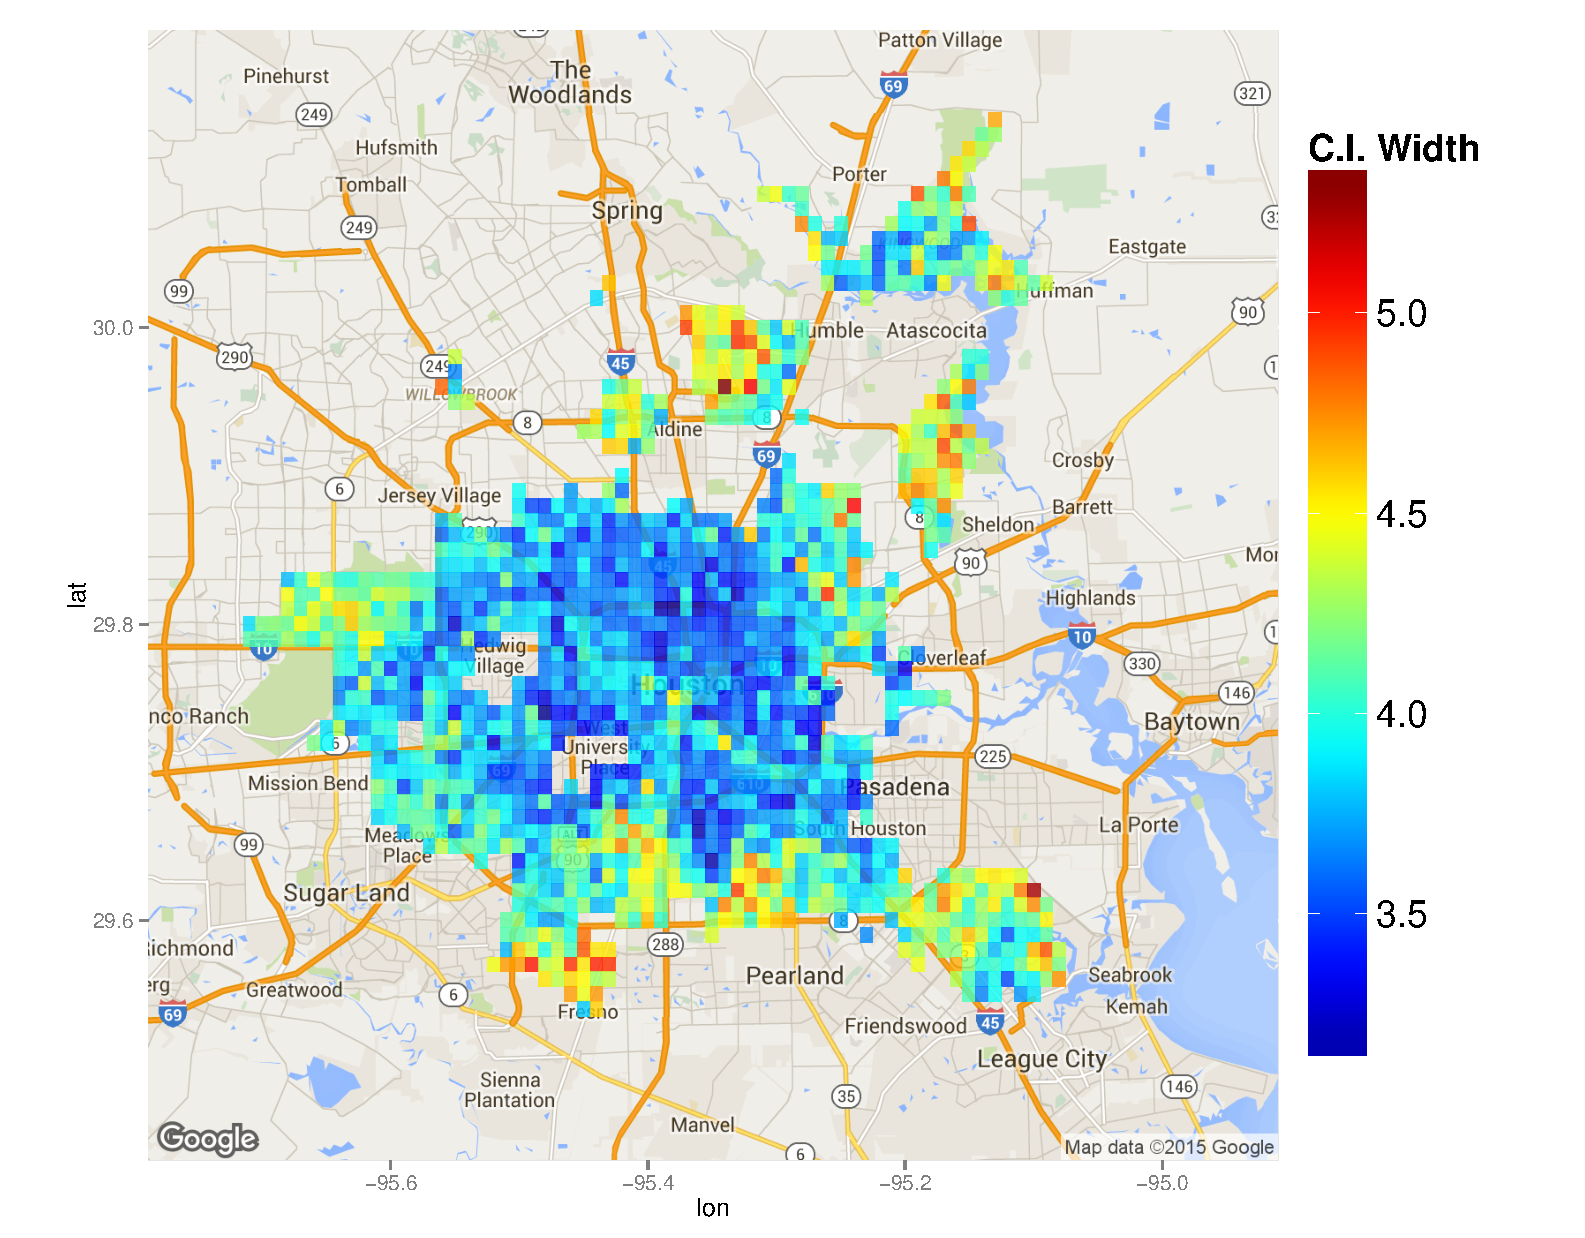
\includegraphics[width=1.0\textwidth]{imgs/overall_ciwidths.pdf}
    f) 95\% CI Widths for Overall Relative Risk
%     \label{rr-overall-ci}
  \end{minipage}
  \caption{Log relative risk maps and 95\% HPD credible interval (CI) widths for 911 calls, mortalities, and overall risk. The spatial distribution for the different health outcomes is obviously different, but the map of the overall relative risks shows evidence that information was successfully borrowed from both health outcomes.}
  \label{relative_risks}
\end{figure}

In Table 2
%\ref{tab:beta_coeff}
 we see the estimates for the $\boldsymbol\beta$ coefficients estimated as part of the mean of $\boldsymbol\mu$. None of the associated credible intervals contain zero, and so we conclude that each of the variables included in this mean has a statistically significant relationship with the average relative risk across all health outcomes. We see that each of the variables considered has a positive relationship with relative risk, and that as average heat index, percent of people in a grid cell over 65, and the number of people without central air conditioning in a grid cell all increase, so does the average relative risk. These effects come as no surprise: examination of the demographic variables in Section \ref{sec:demo_vars} shows that heat-related mortalities were much more likely to occur for people older than 65, and further, as our response variables are associated with extreme heat, it makes sense that as heat increases or the ability to mitigate the effects of heat decreases (fewer people with air conditioning) the incidence of negative health outcomes associated with increased levels of heat should also increase. 

% % Table created by stargazer v.5.2 by Marek Hlavac, Harvard University. E-mail: hlavac at fas.harvard.edu
% % Date and time: Tue, Nov 03, 2015 - 12:25:29
\begin{table} %\centering 
  \caption{$\beta$ coefficients for variables. Because none of the credible intervals contain 0, we conclude that each variable has a significant effect.} 
  \label{tab:beta_coeff} 
\begin{tabular}{@{\extracolsep{5pt}} ccc} 
\\[-1.8ex]\hline 
\hline \\[-1.8ex] 
Variable & $\beta$ &  95\% HPD Credible Interval \\ 
\hline \\[-1.8ex] 
Intercept & $$-$26.378$ & $(-35.268, -15.397)$ \\ 
Average Heat Index & $0.622$ & $(0.356, 0.842)$ \\ 
\% Over 65 & $8.394$ & $(4.851, 12.237)$ \\ 
No Air Conditioning & $0.004$ & $(0.003, 0.006)$ \\ 
\hline \\[-1.8ex] 
\end{tabular} 
\end{table}  

\subsection{Demographic Variables}\label{sec:demo_vars}

Estimation of $\boldsymbol\alpha_p$, $\boldsymbol\gamma_p$, and $\boldsymbol\xi_p$ reveals some distinct differences between the subpopulations experiencing the two different health outcomes in our model. To begin with, Table 3
%$\ref{gendertab}$ 
shows that while heat-related mortalities are slightly more likely to occur to females than males ($0.51$ versus $0.49$), the probability of a heat-related 911 call occurring for a male is about $0.68$ compared to a probability of just $0.32$ for women. Examination of Table 4 %$\ref{ethnicitytab}$% 
reveals that population differences between the health outcomes are not limited to gender. The probabilities that a heat-related mortality occurs for an Asian, black, Hispanic or white individual are $0.02$, $0.36$, $0.11$ and $0.5$, respectively. Conversely, the comparable probabilities of a heat-related 911 call taking place are $0.02$, $0.46$, $0.26$, and $0.27$.  Figure $\ref{pp-age}$ shows that the probabilities for our last demographic variable, age, also differ greatly by health outcome, with the largest $\xi_{911}$ values occurring between 25 and 50, compared with the largest $\xi_{\text{Mort}}$ values clearly occurring above 75. We can also see that while it is extremely rare for a young child to experience a heat-related mortality the probability is much higher for 911 calls suggesting that while young children experience adverse effects from extreme heat they are unlikely to result in death. 

Estimation of the effects of these demographic variables allows us to develop a profile for the type of person most likely to be impacted by extreme heat in a way that results in a specific health outcome. For example, we would expect heat-related mortalities to occur most often for white men and women older than 75 years while we expect heat-related 911 calls to occur most frequently for black males between 25 and 50 years old. These differences show that the effects of extreme heat are not uniform across a population and provide additional evidence that modeling multiple health outcomes, as we've done here, is a necessary step in understanding the total health impact of heat. 

\begin{table}
  \caption{Posterior probabilities and 95\% HPD intervals for gender categories by health outcome. Notice that for a given 911 call the probability that it occurred for a male is much higher than for a female whereas when looking at mortalities the probabilities that a given mortality occurred for a male or female are nearly equal.}
  \label{gendertab}
    \centering
    \begin{tabular}{@{\extracolsep{5pt}} lcccc}\\[-1.8ex]
    \multicolumn{5}{c}{Gender} \\
    \hline
    \hline \\[-1.8ex]
       & \multicolumn{2}{c}{911 Calls} & \multicolumn{2}{c}{Mortalities} \\
       \hline
       & Value & 95\% HPD Int. & Value & 95\% HPD Int. \\
       \hline
      Female & 0.316 & (0.290, 0.343) & 0.514 & (0.506, 0.522) \\
      Male & 0.684 & (0.657, 0.710) & 0.486 & (0.478, 0.494) \\
      \hline \\[-1.8ex]
    \end{tabular}
\end{table}

\begin{table}
  \caption{Posterior probabilities and 95\% HPD intervals for race/ethnicity categories by health outcome. Notice that while heat related 911 calls occur most frequently among the black population, mortalities occur most frequently among white people.}
  \label{ethnicitytab}
  \centering
    \begin{tabular}{@{\extracolsep{5pt}} lcccc}\\[-1.8ex]
    \multicolumn{5}{c}{Race/Ethnicity} \\
    \hline \hline \\[-1.8ex]
    & \multicolumn{2}{c}{911 Calls} & \multicolumn{2}{c}{Mortalities} \\
    \hline
    & Value & 95\% HPD Int. & Value & 95\% HPD Int. \\
    \hline
    Asian & 0.020 & (0.012, 0.028) & 0.025 & (0.022, 0.027) \\
    Black & 0.458 & (0.429, 0.485) & 0.361 & (0.353, 0.369) \\
    Hispanic & 0.255 & (0.231, 0.280) & 0.114 & (0.109, 0.119) \\
    White & 0.267 & (0.241, 0.291) & 0.501 & (0.493, 0.509) \\
    \hline    
    \end{tabular}
\end{table} 


\begin{figure}
    \centering
    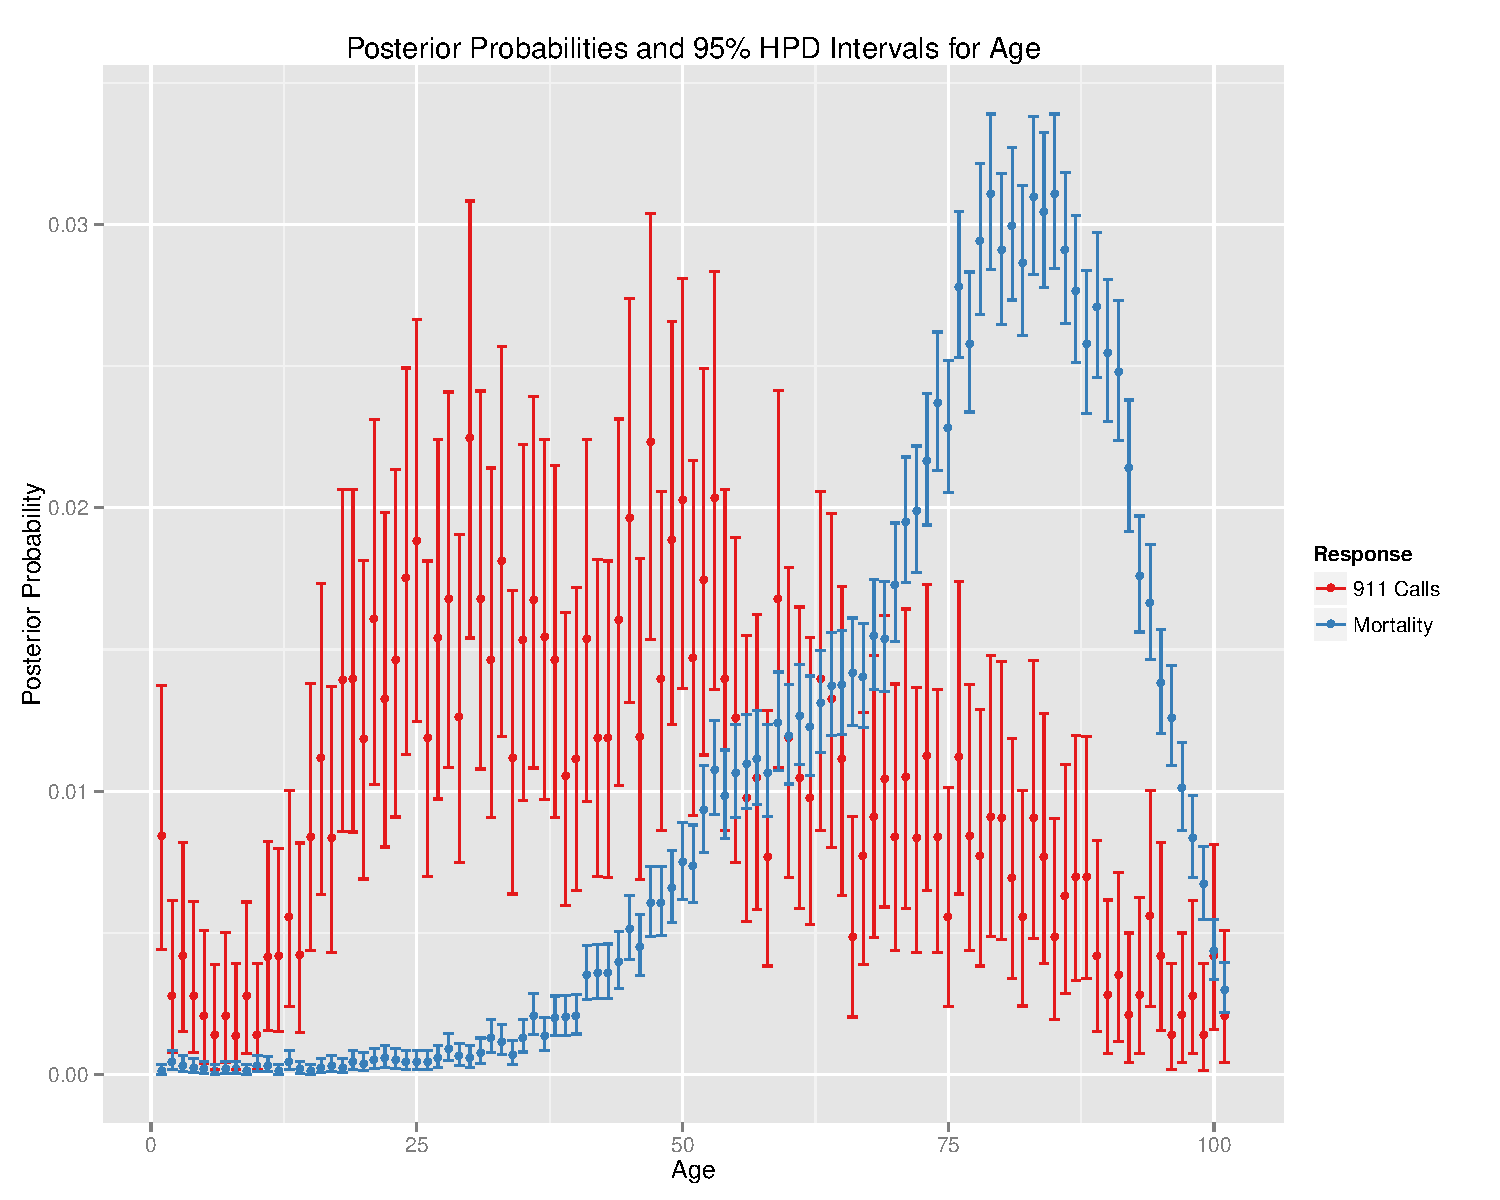
\includegraphics[width=1.0\textwidth]{imgs/pp_age.pdf}
    \caption{Posterior probabilities and 95\% HPD intervals associated with each age by health outcome. Notice that there are distinctly different patterns associated with the different health outcomes, again supporting the idea that it is necessary to consider multiple effects in order to understand the total impact of heat.}
    \label{pp-age}
\end{figure}

\section{Conclusions}
In conclusion, we successfully accomplished the stated goals of this research. Namely, we modeled the impact of heat on multiple health outcomes, calculating and mapping intensity surfaces for each outcome individually as well as estimating and mapping the overall mean intensity surface. Our discretized approach to intensity surface modeling in Equation \eqref{lambda} provided a computationally simple approach that avoided calculation of a random integral.  Examination of correlations showed that the mean intensity surface successfully borrowed information from both data sources and provides evidence that it is an accurate representation of the cumulative effect of heat. Further, we provided uncertainty estimates associated with each surface, allowing for greater precision when using these risk maps to make decisions about which areas are of greatest public health concern. While it has previously been possible to create a kind of overall risk map by simply aggregating data from various health outcomes, the ability to generate an overall risk map in a systematic, model-based fashion is a valuable contribution. 

In addition to estimating the spatial effect of heat on health, we also estimated the probabilities of a health outcome occurring for specific demographic variables and showed distinct differences in how heat affected different subpopulations. These differences emphasize the significance of our research. By combining multiple health outcomes into a single model we are able to understand the impacts of heat in a way that is not captured by any single measure. 

While this research includes interesting first steps towards effectively merging multiple health outcomes, one issue not addressed herein (which is not well-addressed for all point process models) is the assessment of model goodness of fit. Other than post-hoc comparisons between maps of the observed data and maps of the intensity surfaces for the various health outcomes, there is no standard way to determine how well the model fits the data although work by \citet{leininger2014bayesian} suggests this is an active area of research. Another unaddressed issue is that throughout this analysis we treat temperature as fixed by using an average even though temperature is highly variable throughout the summer months. Initially, we attempted to incorporate distributed lag effects \citep{Heaton2012} in this model but found that the data, especially the 911 call data, were too temporally sparse to estimate these effects well.  Thus, developing an effective way to incorporate distributed lag effects and convert this from a purely spatial model to a spatial-temporal one is a potential avenue of further research. 

The practical value of this research becomes apparent as public health officials seek to plan interventions to decrease the negative effects of extreme heat. Being able to consider and identify the areas that are most adversely affected across all negative health outcomes, instead of just one, can help to target resources in areas that are affected most heavily, leading to more effective and efficient responses to extreme heat.


\bibliographystyle{rss}
\bibliography{bibliography}

\end{document}
